\documentclass[acmtog, authorversion]{acmart}
\usepackage{graphicx}
\usepackage{minted}
%\usepackage[numbers]{natbib}
\usepackage{float}
%\usepackage{hyperref}
%\usepackage{comment}
%\usepackage{ragged2e}
\setcopyright{none}
\citestyle{acmauthoryear}

\sloppy
\begin{document}
\title{Járművek trajektóriájinak előrejelzése machine learning modellekkel}

\author{Péter Bence Mérnökinformatika BSc 6. félév}%\\Mérnökinformatika BSc 6. félév\\Konzulensek:\\Dr. Horváth András egyetemi docens\\Agg Áron PhD hallgató}
\authornotemark[1]
\affiliation{
    \institution{Széchenyi István Egyetem}
    \city{Győr}
    \country{Hungary}}

\author{Dr. Horváth András}
\affiliation{
    \institution{Széchenyi István Egyetem}
    \city{Győr}
    \country{Hungary}}

\author{Agg Áron PhD hallgató}
\affiliation{
    \institution{Széchenyi István Egyetem}
    \city{Győr}
    \country{Hungary}}

\begin{teaserfigure}

\includegraphics[width=1\columnwidth]{sze_givk_logo.png}
\Description{egyetem_kar}
\end{teaserfigure}

\begin{abstract}
    Az ITS (intelligent transportation system) egyre nagyobb teret 
    hódít napjainkban és rengeteg különböző területen alkalmazzák 
    ezeket a rendszereket. A közlekedési csomópontok elemzése egy 
    frekventált terület az ITS alkalmazásában.
    Célunk, gépi látás és gépi tanulás felhasználásával, közlekedési
    csomópontok elemzésének automatizálása és felgyorsítása. A kutatásban
    lefektetett alapgondolatokat, kifejlesztett keretrendszert és 
    a felmerülő probélmák megoldásait, a gyakorlatban balesetek megelőzésére,
    renitens viselke-dések kiszűrésére és forgalomirányító renszerek támogatásá-ra
    lehet használni.  
    A kutatásban egy trajektória osztályozó módszert ismertetünk, amely objektumdetektálás 
    és objektumkövetés segítségé-vel elemezi a közlekedési 
    csomópontokban elhaladó járművek mozgá-sát. A mozgásuk alapján 
    klaszterezi a trajektóriákat, majd gépi tanulás 
    segítségével predikciót ad az újonnan belépő járművek kilépési 
    pontjára. A módszerhez 6 különböző közlekedési csomópont-ban 
    készített saját videó adatbázisunkat használtuk fel.
    A tesztelt klaszterezési mód-szerek közül (OPTICS, BIRCH, KMeans, DBSCAN)
    az OPTICS algoritmus bizonyult legjobbnak trajektórák klaszterezésére.
    Összehasonlí-tottunk több különböző klasszifikációs módszert 
    a legpontosabb predikció eléréséhez, amelyek: KNN, SVM, GP, DT, 
    GNB, MLP, SGD. A tanul-mányban bemutatott eljárások közül az 
    KNN adta atlagban a legpontosabb 90\%-os eredményt.
    %Ezt a pontosságot valós idejű futás közben 5 fps mellett érte el.
    %Ebből azt a következtetést lehet levonni, hogy jobb sebesség elérése
    %érdekében, vagy a feature vectorok dimenzióját kell csökkenteni, vagy
    %érdemes neurális hálót alkalmazni a klasszifikációhoz.
    %A forráskód megtalálható ebben a github repositoriban 
    %\url{https://www.github.com/Pecneb/computer_vision_research}
\end{abstract}

\maketitle

\tableofcontents

\section{Bevezetés}
A városok növekedése egyre nagyobb forgalomhoz vezet, ami a balesetek, forgalmi dugók számát növeli és a levegő minősége is romlik.
Az ITS (intelligent transportation system) fejlesztése a városokban erre megoldást jelenthet. Ez magába foglalja az információs és
kommunikációs technológiák, mint pélául szenzorok, kamerák, kommunikációs hálózatok és adat elemzés fejlesztését. 5G hálózatokon
keresztül, ezek a technológiák összeköthetők a közlekedési eszközökkel. Ehhez okos forgalomirányítási rendszerek kifejlesztésére
van szükség, amik információval tudnak szolgáni a járművekbe szerelt informatikai rendszereknek.
A legértékesebb információt a közlekedésben részvevő járművek jelen és jövőbeli pozíciója jelenti. Pontos és gyors trajektória 
előrejelző rendszerek kifejlesztése egy nagy kihívás és egyre növekszik irántuk a kereslet. E kutatási terület kiforratlanságából
eredően, kevés létező keretrendszer és adathalmaz található, így a tanító adathalmaz gyűjtése, adatok kinyerésének formátuma, tárolása
és mérőszámok kifejlesztése (amivel a tesztelni kívánt modellek pontosságát tudjuk mérni) is a kutatáshoz tartoznak.  
Ebben a kutatásban erre a problémára törekszünk egy módszertant és keretrendszert kifejleszteni, emellett klaszterezési és klasszifikációs
algoritmusokat tesztelni. A tanító adatok előállításához, objektumok detektálására a YOLOv7 \cite{wang2022yolov7}
konvolúciós neurális hálót használtuk, ez a konvolúciósl neurális háló architektúra nem csak nagy pontosságot hanem sebességet is nyújt nekünk. 
Emellett képkockáról képkockára követni is kell tudni a detektált objektumokat. Erre is sok megoldás található manapság, erre a feladatra
a DeepSORT \cite{Wojke2018deep} nevezetű algoritmust használtuk, ez kálmán filtert és konvolúciós neurális hálót használ az objektumok követésére.
A tanító adatok 6 különböző helyszín forgalmát tartalmazzák. Minden helyszín más tulajdonságokkal bír, ezért nem lehet generalizálni
a tanítási folyamatot, nem lehet egy univerzális modellt betanítani ami minden közlekedési helyszínre alkalmazható egyaránt. A klaszterezés
során megpróbáljuk minél pontosabban meghatározni a be és kimeneti pontok által leírt klasztereket, amelyek majd alapul szolgálnak a
klasszifikáció tanítása során. Több fajta klaszterezési algoritmust megvizsgáltunk a kutatás során, KMeans, OPTICS \cite{10.1145/304181.304187}, BIRCH \cite{10.1145/233269.233324} és DBSCAN \cite{10.5555/3001460.3001507}\cite{10.1145/3068335}. 
A klasszifikációhoz bináris klasszifikációs modelleket kombinálunk, így több osztályos klasszifikációs modelt
kapunk. Minden bináris modelnél, egy osztály az összes többivel szemben van betanítva. A modellek pontosságának kiértékelésére 3 mérőszámot
alkalmaztunk, amik az \emph{Accuracy Score}, \emph{Balanced Accuracy Score} \cite{10.1109/ICPR.2010.764} és \emph{Top-k Accuracy Score}.
Mindegyik mérőszám kiszámolásához \emph{K-Fold Cross-Validation} \cite{Anguita2012TheI} metódust alkalmaztunk, ahol \begin{math}K=5\end{math}.

\section{Kapcsolódó kutatások}
Sok ITS-el kapcsolatos kutatásban tárgyalják a forgalom folyás (traffic flow) előrejelzését. \cite{PAUL2017177} össze-hasonlítja az eddig
kutatott és használt modellek, mint például Kalman Filtering, k-nearest neighbor (k-NN), mesterséges neurális hálók, stb., pontosságát és
sebességét, ezen modellek tovább-kutatását, mivel egyre növekednek a különböző szenzorok által  begyűjtött traffic flow adatok, így ez a terület belépett
a \emph{Big Data} korszakába. \cite{10.1371/journal.pone.0253868} is a traffic flow előrejelzését és generálását tárgyalja, Floating Car Data (FCD) 
adathalmazokon betanított, Hosszú-Rövid-Távú memóriájú és Generatív versengő hálókkal.
\subsection{YOLO}
"You look only once" (YOLO) egy state-of-the-art, valós idejű objektum detektáló rendszer. Legfrissebb változata a Yolov7 felülmúlja sebességben
és pontosságban a modern konvolúciós hálókat (lásd \ref{fig: Yolov3chart} \ref{fig: Yolov4chart} \ref{fig: Yolov7chart}). Beágyazott rendszerekben és videókártyá-kon is egyaránt jó a teljesítménye, ezért az ITS területén
alkalmazható. 
\begin{figure}[H]
 \Description{YOLOv3 perfomance over other CNN models.}
 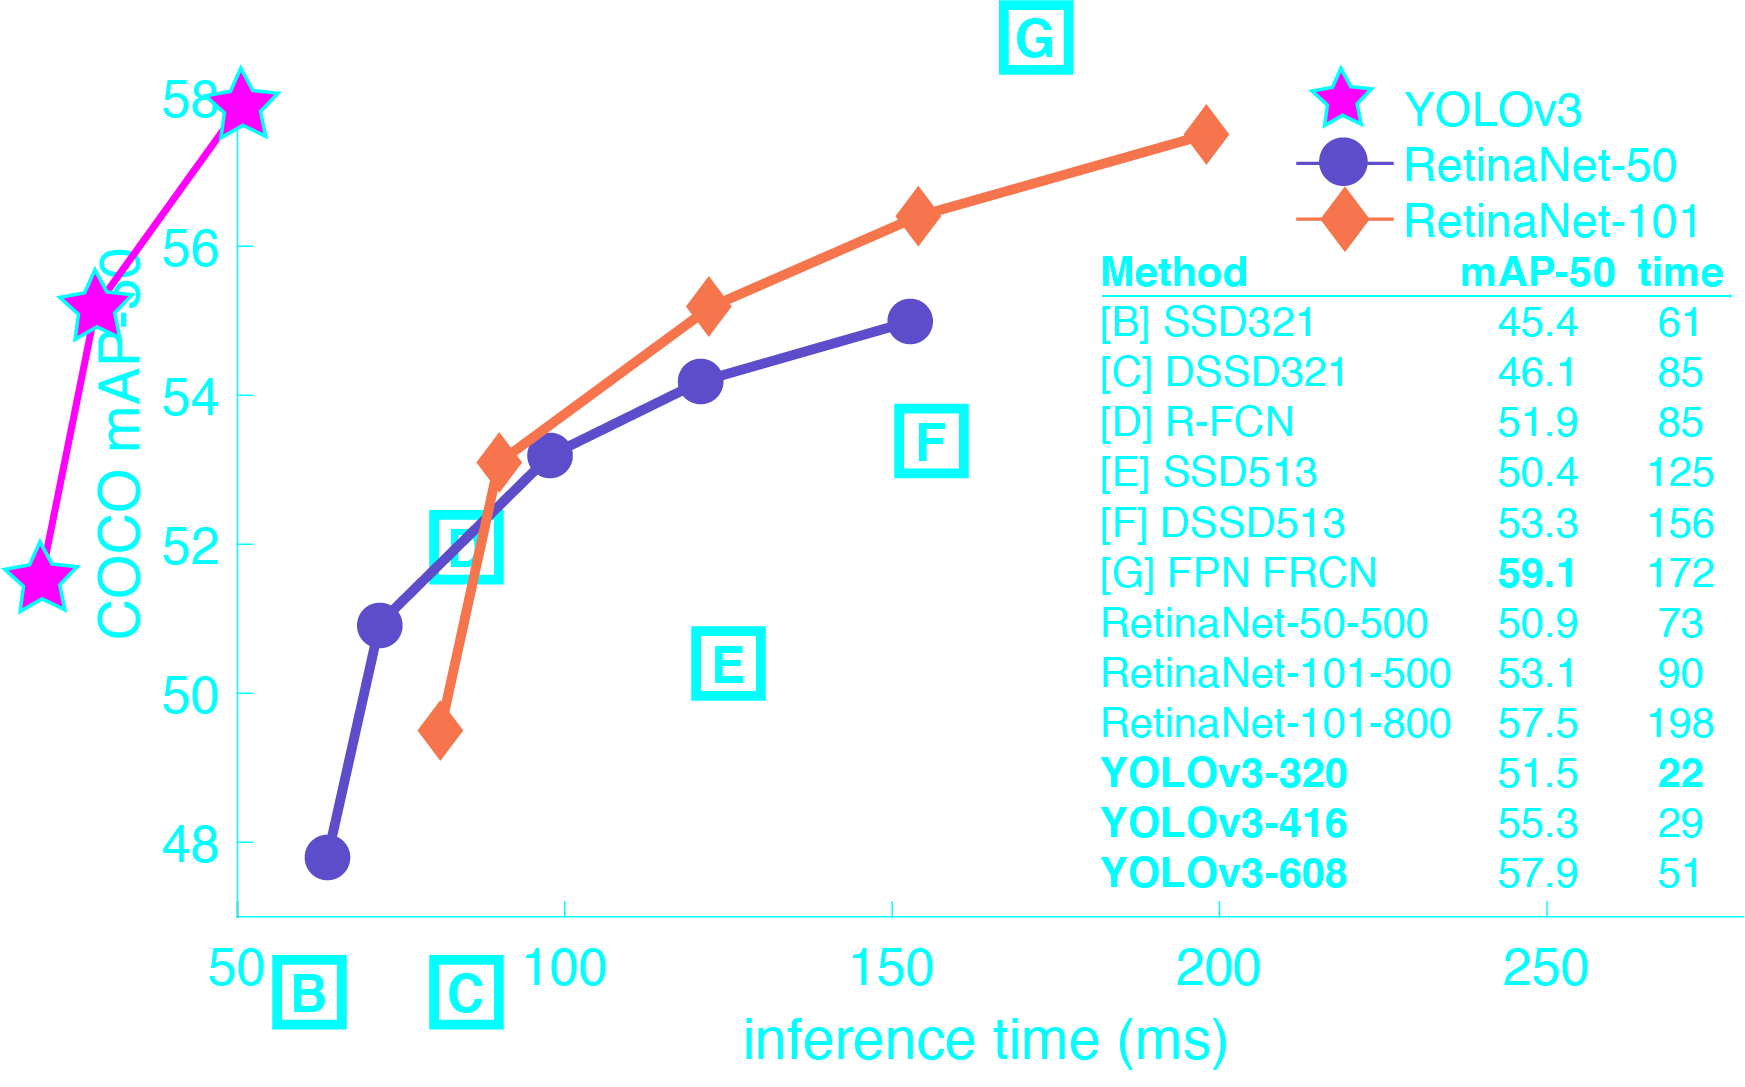
\includegraphics[width=1\columnwidth]{yolov3_perf.png}
 \caption{YOLOv3 Performance}
 \label{fig: Yolov3chart}
\end{figure}
\begin{figure}[H]
 \Description{YOLOv4 perfomance over other CNN models.}
 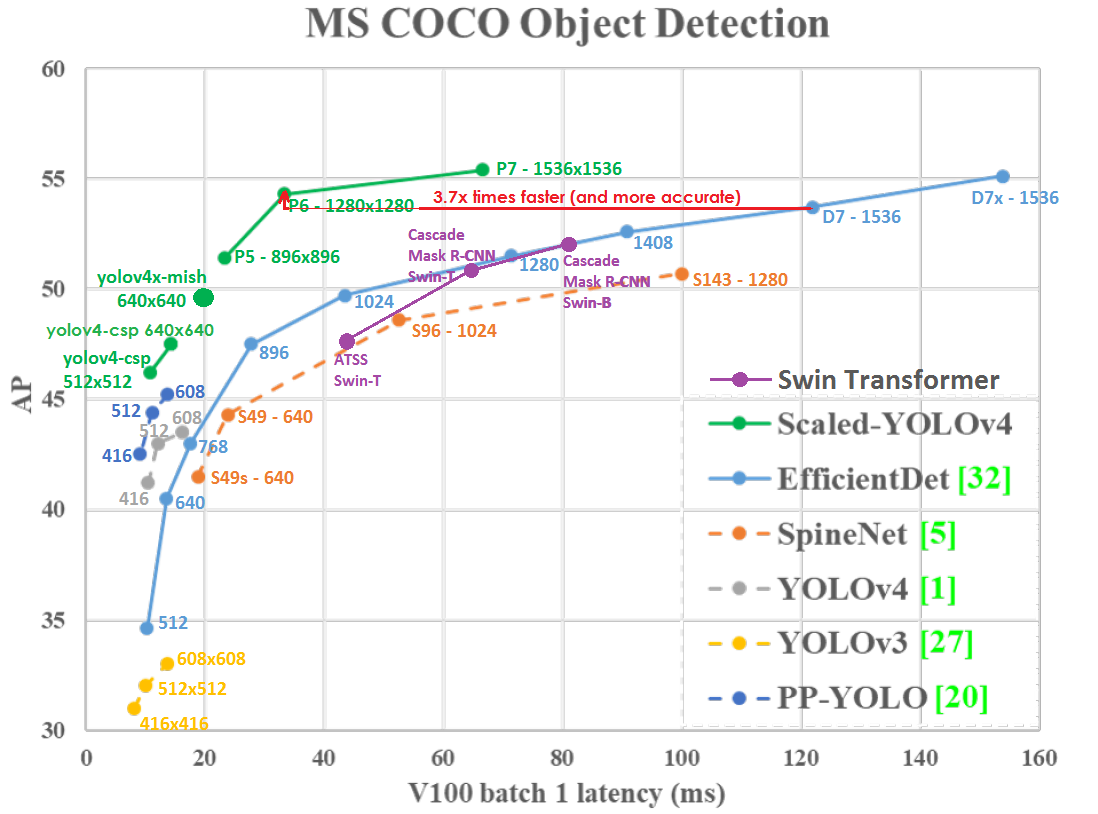
\includegraphics[width=1\columnwidth]{yolov4_perf.png}
 \caption{YOLOv4 Performance}
 \label{fig: Yolov4chart}
\end{figure}
\begin{figure}[H]
 \Description{YOLOv7 perfomance over other yolo models.}
 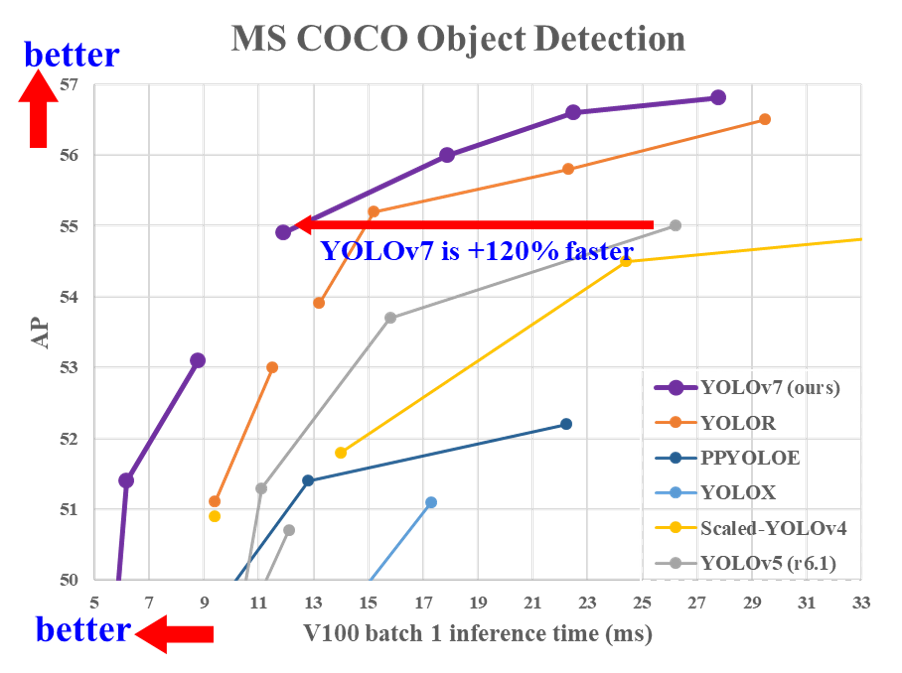
\includegraphics[width=1\columnwidth]{performance.png}
 \caption{YOLOv7 Performance}
 \label{fig: Yolov7chart}
\end{figure}
\subsection{DeepSORT}
Simple Online and Realtime Tracking with a Deep Association Metric (DeepSORT) a SORT algoritmus egy továbbfejlesztett változata. Az eredeti
algoritmus sebességét törekednek növelni egy offline tanítási lépéssel. A betanított mély asszociációs metrika segítségével nagyban lecsökkentették
az identitás vál-tásokat, és hosszabb elfedés után is követni tudja az objektumokat.

\section{Adathalmazok kialakítása}
A kutatás során saját adathalmazok kialakítására volt szükség. Az adatok begyűjtésére és eltárolására saját alkalmazást és keretrendszert
fejlesztettünk ki. A szoftver keretrendszert python nyelven írtuk meg, a forráskód ezen a linken megtatlálható \url{http://github.com/Pecneb/computer_vision_research}.
A fejlesztés során a következő programkönyvtárakat használtuk OpenCV \cite{opencv_library}, Numpy \cite{harris2020array}, Pandas \cite{reback2020pandas}, 
Scikit-Learn \cite{scikit-learn}, Matplotlib \cite{Hunter:2007}, SQLite \cite{sqlite2020hipp}, Joblib \cite{joblib_library}. Az adat-halmazokat SQLite adatbázisban és
joblib fájlokban tároltuk el. Azért döntöttünk így, hogy két féle módon is eltároljuk az adathalmazokat, mert az SQL adatbázist univerzálisan
bármilyen adatbáziskezelővel, vagy más programnyelvvel be lehet olvasni, viszont a joblib fájlokat sokkal gyorsabban be lehet töletni pythonnal.
\subsection{Adatstruktúra}
Az adatstruktúrát SQL schema-ként, és python class-ként is definiáltuk.
\begin{minted}{sql}
CREATE TABLE IF NOT EXISTS objects (
            objID INTEGER PRIMARY KEY NOT NULL,
            label TEXT NOT NULL
        );
CREATE TABLE IF NOT EXISTS detections (
            objID INTEGER NOT NULL,
            frameNum INTEGER NOT NULL,
            confidence REAL NOT NULL,
            x REAL NOT NULL,
            y REAL NOT NULL,
            width REAL NOT NULL,
            height REAL NOT NULL,
            vx REAL NOT NULL,
            vy REAL NOT NULL,
            ax REAL NOT NULL,
            ay REAL NOT NULL,
            vx_c REAL NOT NULL,
            vy_c REAL NOT NULL,
            ax_c REAL NOT NULL,
            ay_c REAL NOT NULL,
            FOREIGN KEY(objID) REFERENCES objects(objID)
        );
CREATE TABLE IF NOT EXISTS metadata (
            historyDepth INTEGER NOT NULL,
            yoloVersion TEXT NOT NULL,   
            device TEXT NOT NULL,
            imgsize INTEGER NOT NULL,
            stride INTEGER NOT NULL,
            confidence_threshold REAL NOT NULL,
            iou_threshold REAL NOT NULL,
            k_velocity REAL NOT NULL,
            k_acceleration REAL NOT NULL
        );
\end{minted}
Minden követett objektum egyedi azonosítóval lett ellátva. Az objektumhoz tartozó detektálások külön táblába lett kiszervezve,
ahol az \textit{objID} idegen kulcsal kapcsoljuk az \textit{objektumok} táblához. Egy objektumhoz az egyedi azonosítón kívül
tartozik egy \textit{label} amit a YOLO objektum detektálótól kap, ez lehet pl. autó, személy, teherautó, stb. Az objektumokhoz
tartózó detektálások tartalmazzák a képkocka számát, amikor a detektálás történt, a konfidenciát, hogy mennyire biztos az
objektumfelismerő a hozzárendelt \textit{label}-ben, az objektum \begin{math}X,Y\end{math} kordinátáját, az objektum szélességét
\begin{math}width\end{math} és magasságát \begin{math}width\end{math}, sebességét \begin{math}v_x,v_y\end{math} és gyorsulását \begin{math}a_x,a_y\end{math}, 
amik a deepSORT által kalkulált értékek, így még külön a koordinátákból kiszámolt \begin{math}v_{x_c},v_{y_c}\end{math} sebességet és
\begin{math}a_{x_c},a_{y_c}\end{math} gyorsulást is eltároltuk.
Ezek mellett még a konfigurációs adatokat is külön táblában tároljuk, hogy később meg lehessen ismételni a detektálást. 
A koordinátákat a videó méretének megfelelően leskálázzuk 0 - 1 értékek köré. Ha a videó kép szélesség \begin{math}w\end{math}, magasság \begin{math}h\end{math}, 
akkor a képarány \begin{math}r = \frac{w}{h}\end{math}, és az eltárolt koordináták \begin{math}X = \frac{X_0}{w} * r\end{math}, \begin{math}Y = \frac{Y_0}{w} * r\end{math},
\begin{math}v_x = \frac{v_{x_0}}{w} \cdot r\end{math}, \begin{math}v_y = \frac{v_{y_0}}{w} * r\end{math}, \begin{math}a_x = \frac{a_{x_0}}{w} * r\end{math}, \begin{math}a_y = \frac{a_{y_0}}{w} * r\end{math}
\begin{math}v_{x_c} = \frac{v_{xc0}}{w} * r\end{math}, \begin{math}v_{y_c} = \frac{v_{yc0}}{w} * r\end{math}, \begin{math}a_{x_c} = \frac{a_{xc0}}{w} * r\end{math}, \begin{math}a_{y_c} = \frac{a_{yc0}}{w} * r\end{math}.
\subsection{Objektumdetektálás}
Az objektumdetektáláshoz a fennt említett YOLO modellt haszáltuk. Kutatásunk kezdetekor, a YOLO 4-es verziójával kezdtünk dolgozni,
de később átváltottunk a jobb pontosságot és sebességet ígérő 7-es verzióra.
\subsubsection{YOLOv4}
YOLO 4-es verzióját, C-ben implementálták. Hogy fel tudjuk használni, írnunk kellett egy python API-t, ami meg tudtunk hívni a
deketáló programunkban.
\subsubsection{YOLOv7}
A YOLOv7 viszont már python-ban implementálták amihez már sokkal könnyebb volt API-t progra-mozni és használni. Emellett, gyorsaságban
és pontosságban is felülmúlta a 4-es verziót (lásd \ref{fig: Yolov7chart}).
\subsection{Objektumkövetés}
Ahhoz, hogy trajektóriák alapján tudjunk szabájosságokat felismerni a forgalomban, pontos objektumkövetésre volt szükségünk. Eleinte
saját objektumkövető algoritmust használ-tunk, ami deketálások euklideszi távolsága alapján próbálta meg követni az objektumokat.
Ezzel az volt a gond, hogy hosszabb kitakarás után nem találta meg az objektumot, így egy új objektumnak számított, ami a kép
közepéből bukkant fel. Ennek a problémának a kiküszöbölésére próbáltuk ki a DeepSORT algoritmust.
\subsubsection{DeepSORT}
A DeepSORT algoritmus pythonban implementált változatát integráltuk a mi programunkba.

\section{Klaszterezés}
A klaszterezés segítségével lehet az adathalmazból alőállítani a klasszifikáció alapjául szolgáló klasszokat. Ahhoz, hogy az
a rengeteg trajektóriából és detektálásból számunkra felhasználható információ keletkezzen, meg kell határoznunk feature
vectorokat, amik a trajektóriákra jellemző értékeket tartalmaznak. Ebben a feature térben fogja a klaszterező algoritmus
megtalálni az egymáshoz közeli, hasonló trajektóriákat.
\subsection{Adattisztítás}
A klaszterezés előtt a nyers adatokat fel kell dolgoznunk, hogy az esetleges hibás, zajos detektálások, trajektóriák miatt
kapjunk fals klasztereket. Az objektum detektálás és követés nem tökéletes, rossz fényviszonyok, hosszabb eltakarások miatt 
a trajektóriák megszakadhatnak, ezért ki kell választani az egyben maradt trajektóriákat. Három szűrő algoritmust futtattunk 
az adathalmazon. Elsőnek a trajektóriák belépő és kilépő pontjainak az euklideszi távolsága alapján szűrtünk.
Majd a kép széleit meghatározzuk min max kiválasztással, és azokat a trajektórákat választjuk ki amiknek a szélektől meghatározott
távolságra vannak a belépő és kilépő pontjaik.
\subsubsection{DeepSORT pontatlanság}
Kutatásunk során azt tapasztaltuk, hogy a DeepSORT és a YOLO pontatlanságai felerősítik egymást. A YOLO hajlamos néha táblákat
vagy rendőr lám-pákat autóknak nézni, és ekkor a DeepSORT is elkezdi követni. Egy olyan hibáját is felfedeztük a DeepSORT-nak, hogy
egy objektumról áttapad a követés egy másik objektumra, ami fals trajektóriákat hoz létre. A DeepSORT-nak lehet finomhangolni A
paramétereit, ami nem bizonyult akkora javulásnak, ezért útólagos szűréssel kellett korrigálnunk ezt a hibát. Az algoritmus végig 
iterál a trajektóriák pontjain és kiszámítja az egymást követő detektálások euklideszi távoláságát, és ha egy küszöbérték felett vannak akkor eldobjuk a trajektóriát.
A következő képeken láthatók a klaszterek szűrés előtt és után (lásd \ref{fig: Klaszterezés szűrő} \ref{fig: Klaszterezés szűrő 2}).

\begin{figure}
 \Description{Klaszter 0 szűrés előtt és után}
 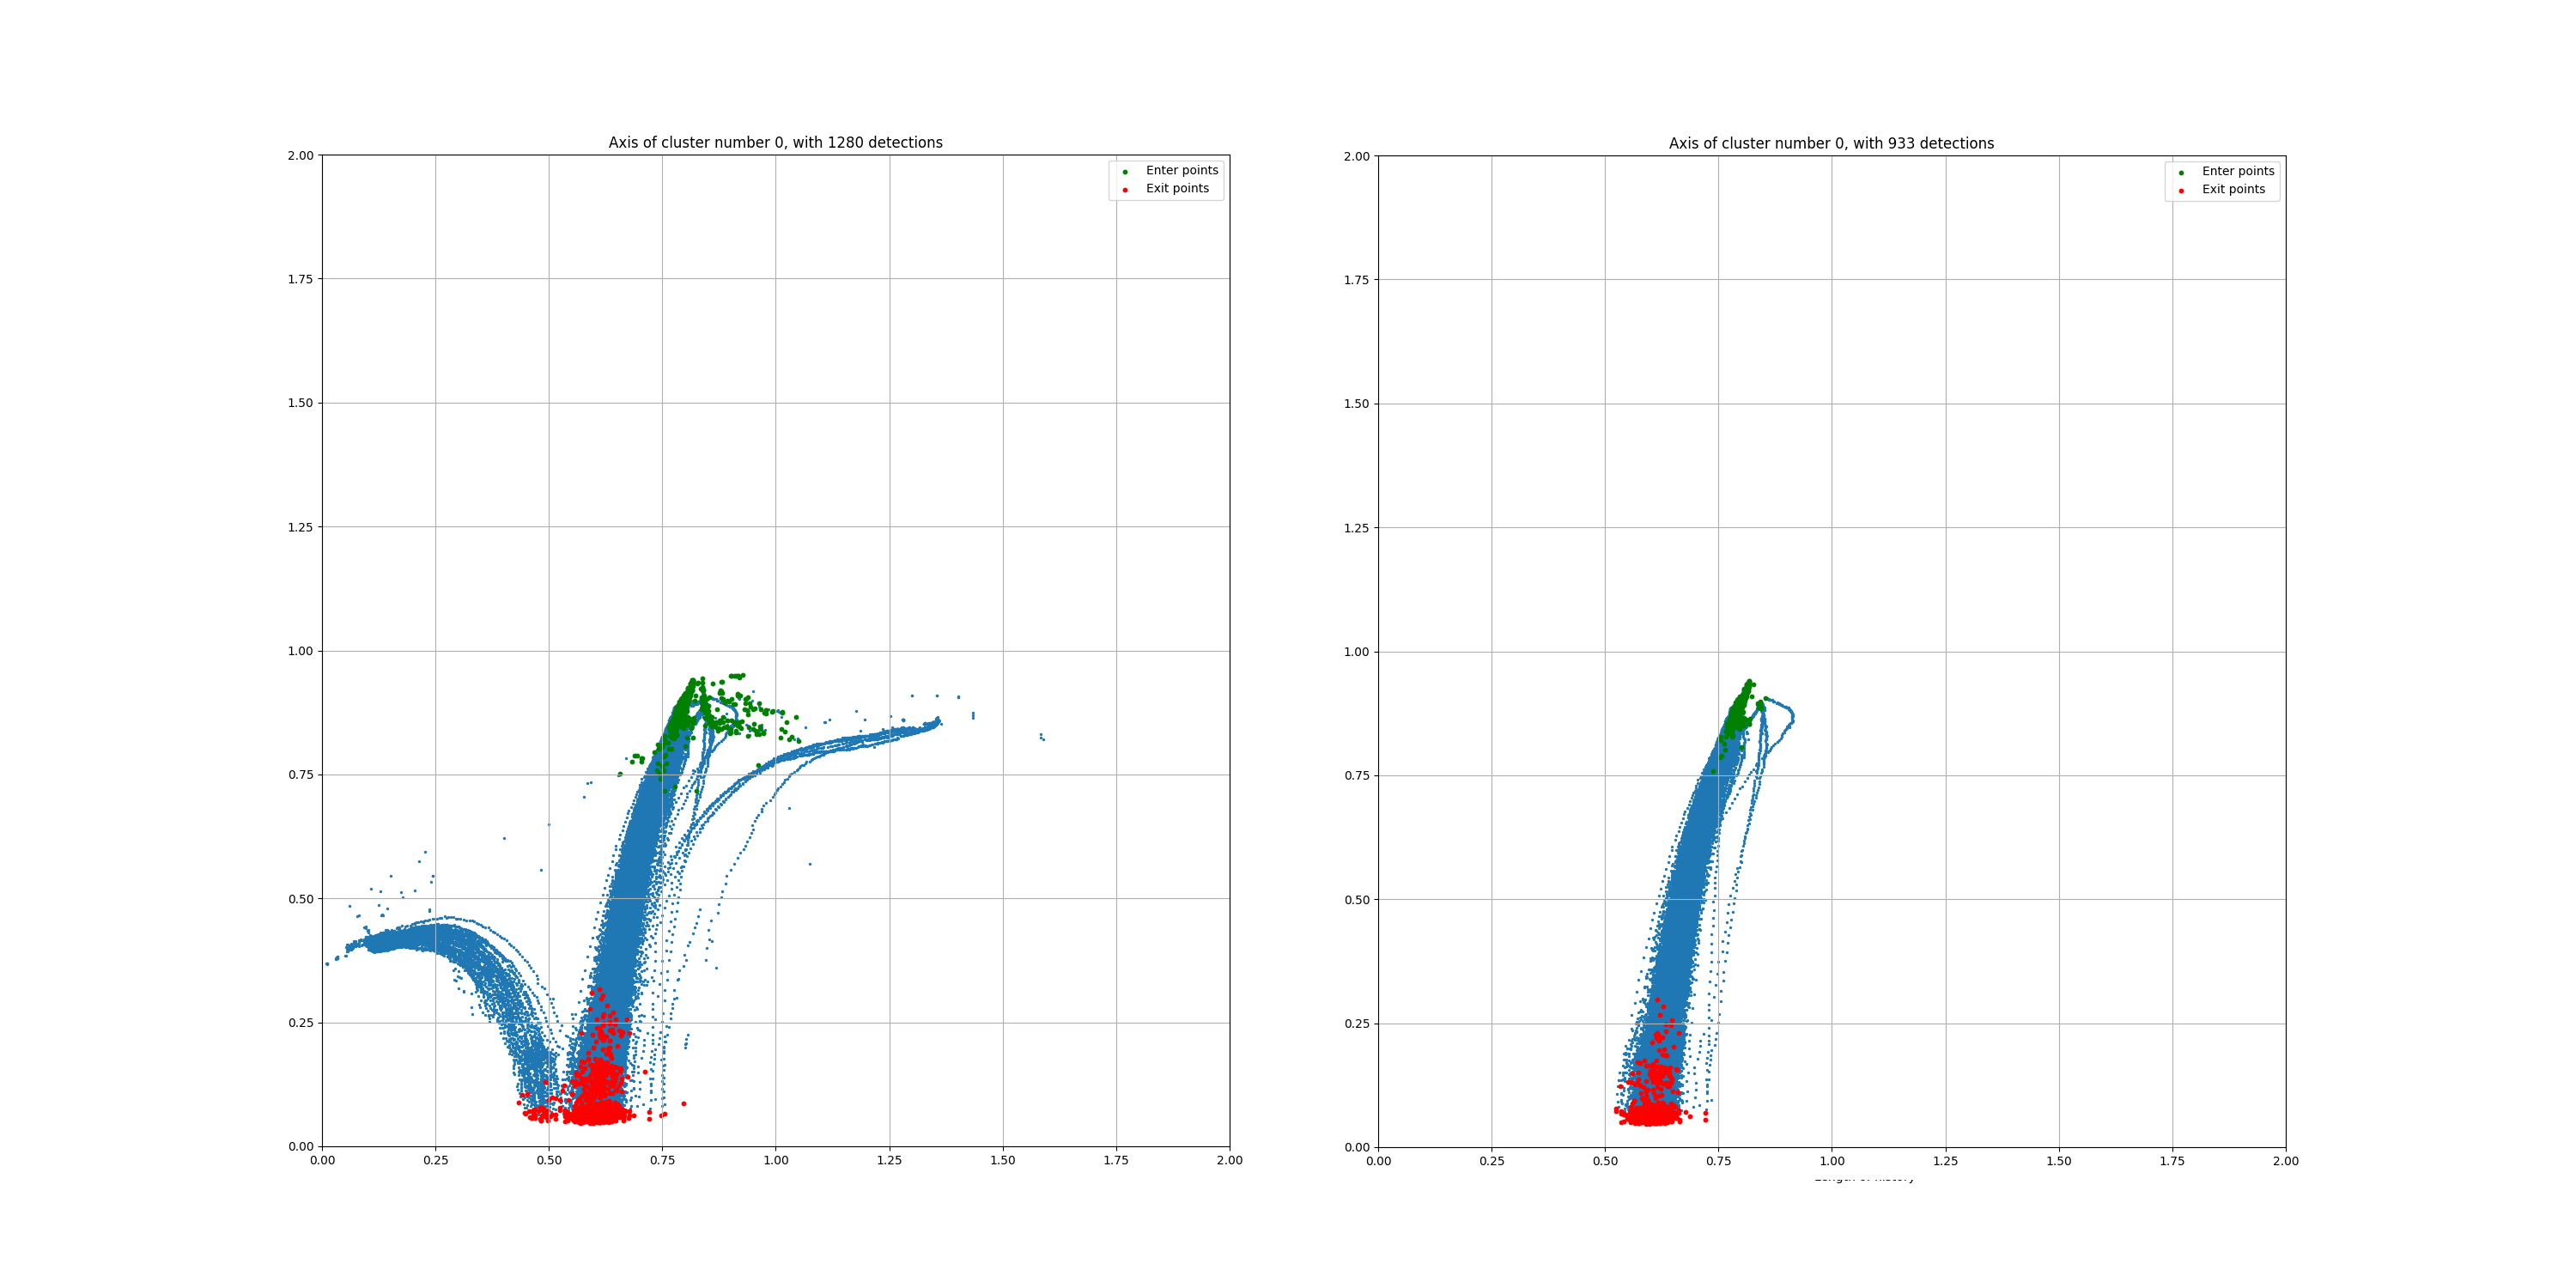
\includegraphics[width=1\columnwidth]{clustering/n_cluster_0_before_after.png}

 \Description{Klaszter 2 szűrés előtt és után}
 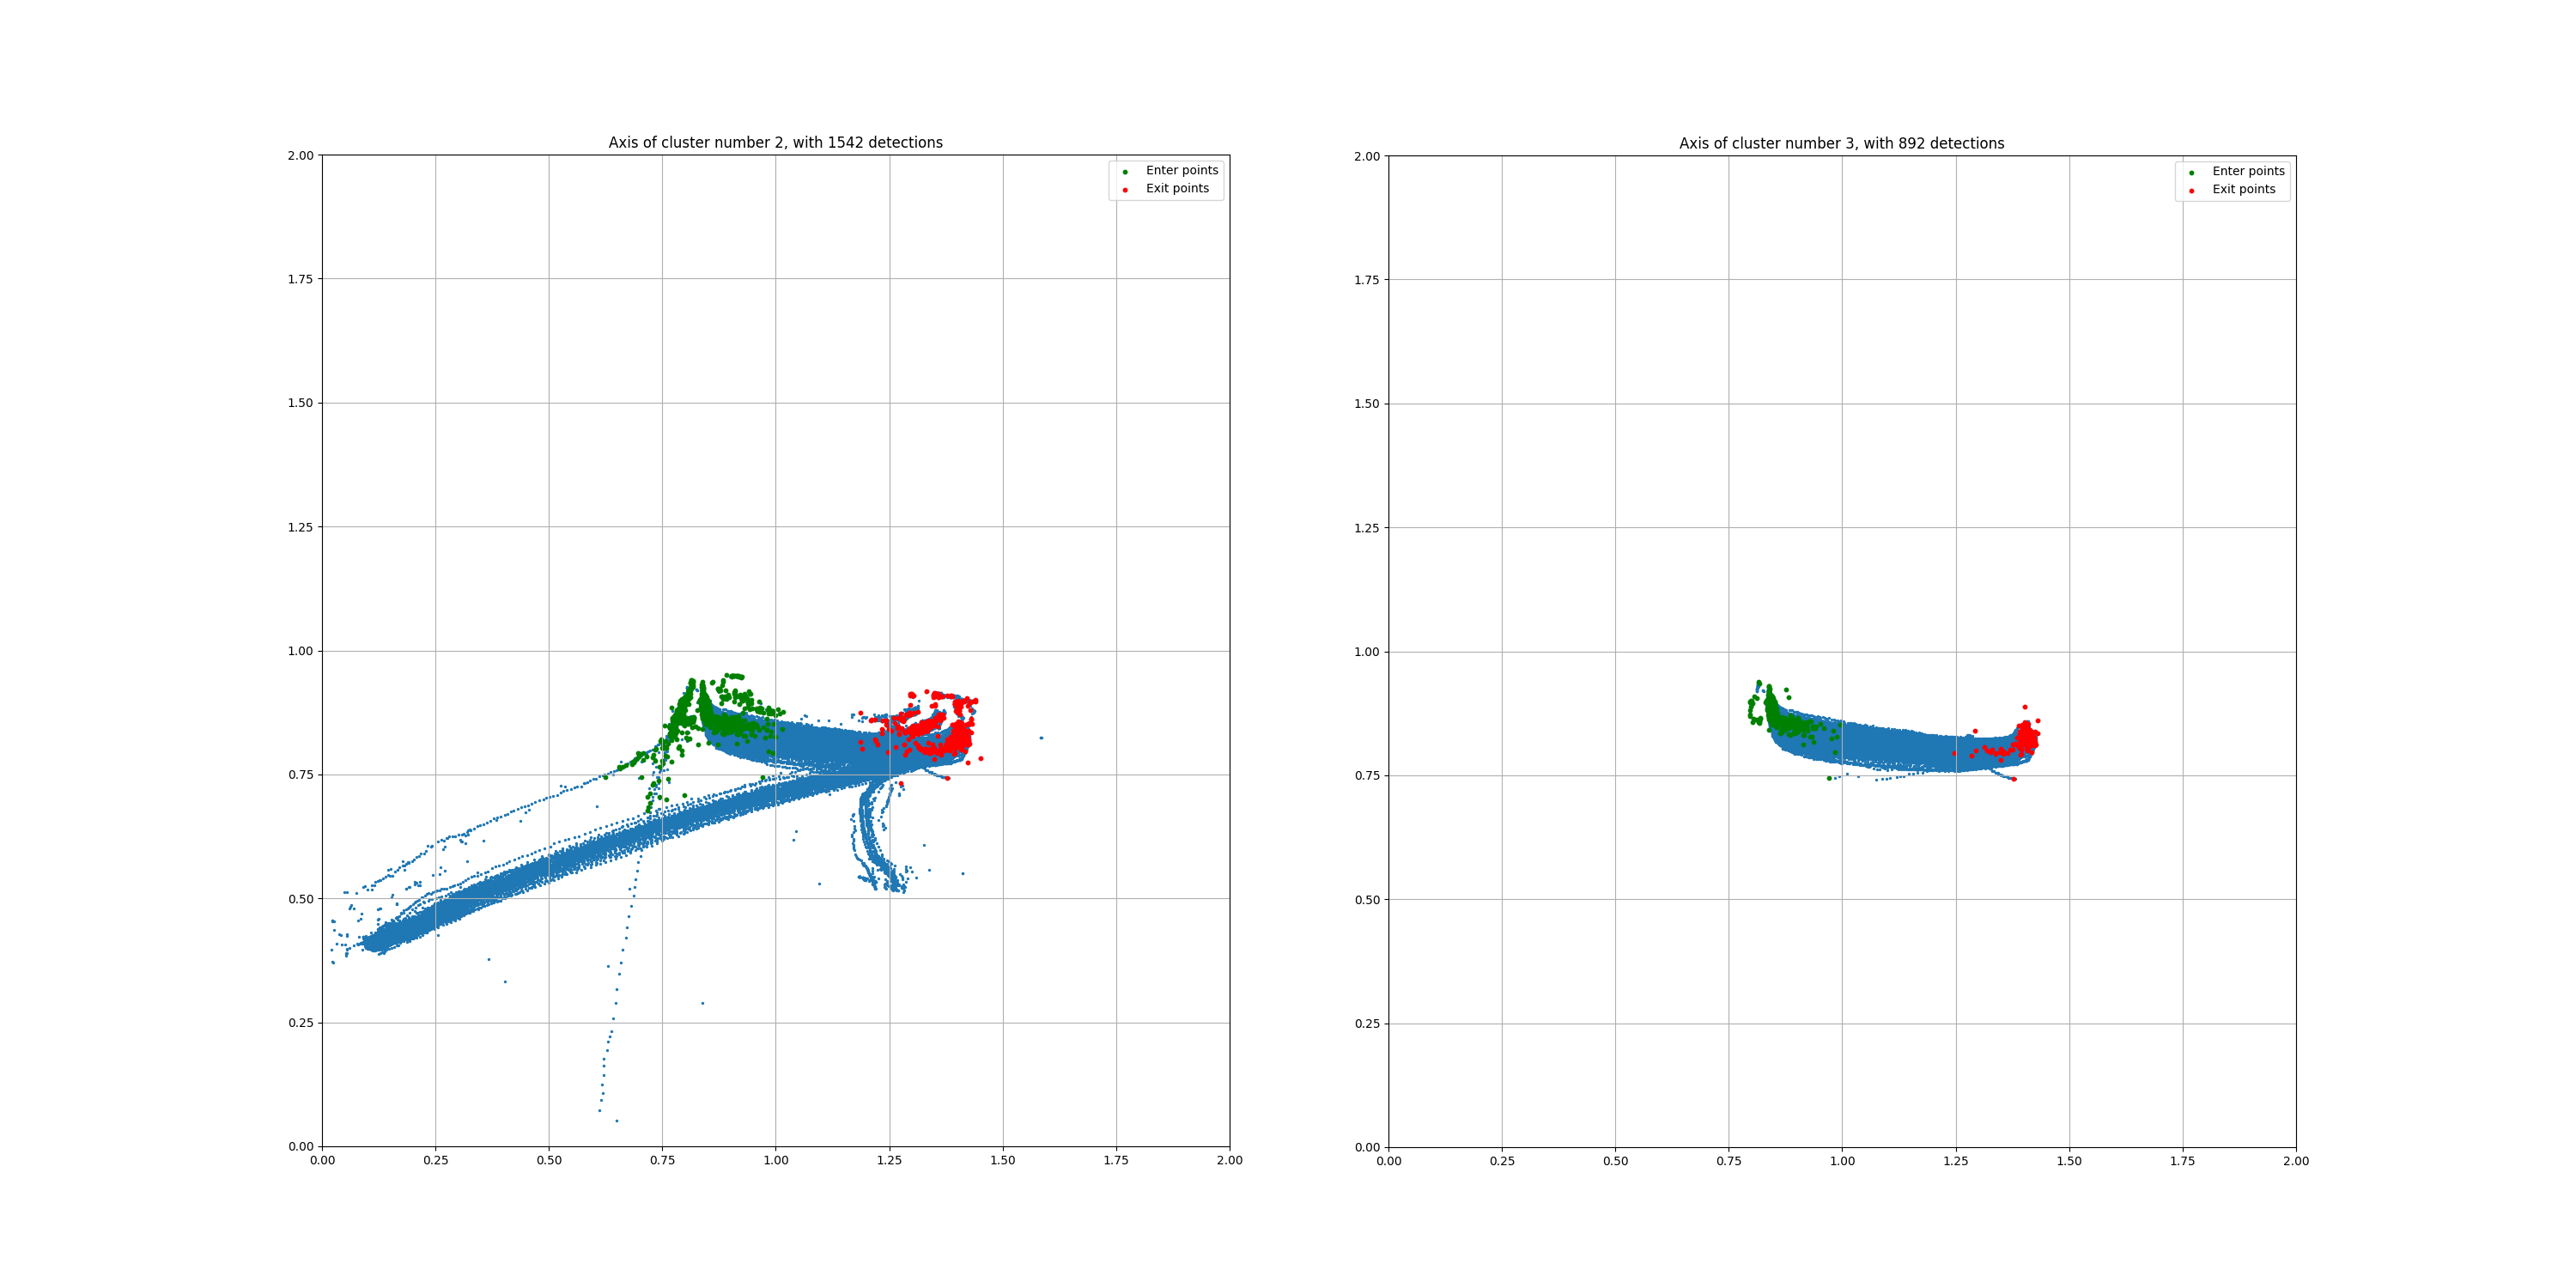
\includegraphics[width=1\columnwidth]{clustering/n_cluster_2_before_after.png}

 \Description{Klaszter 3 szűrés előtt és után}
 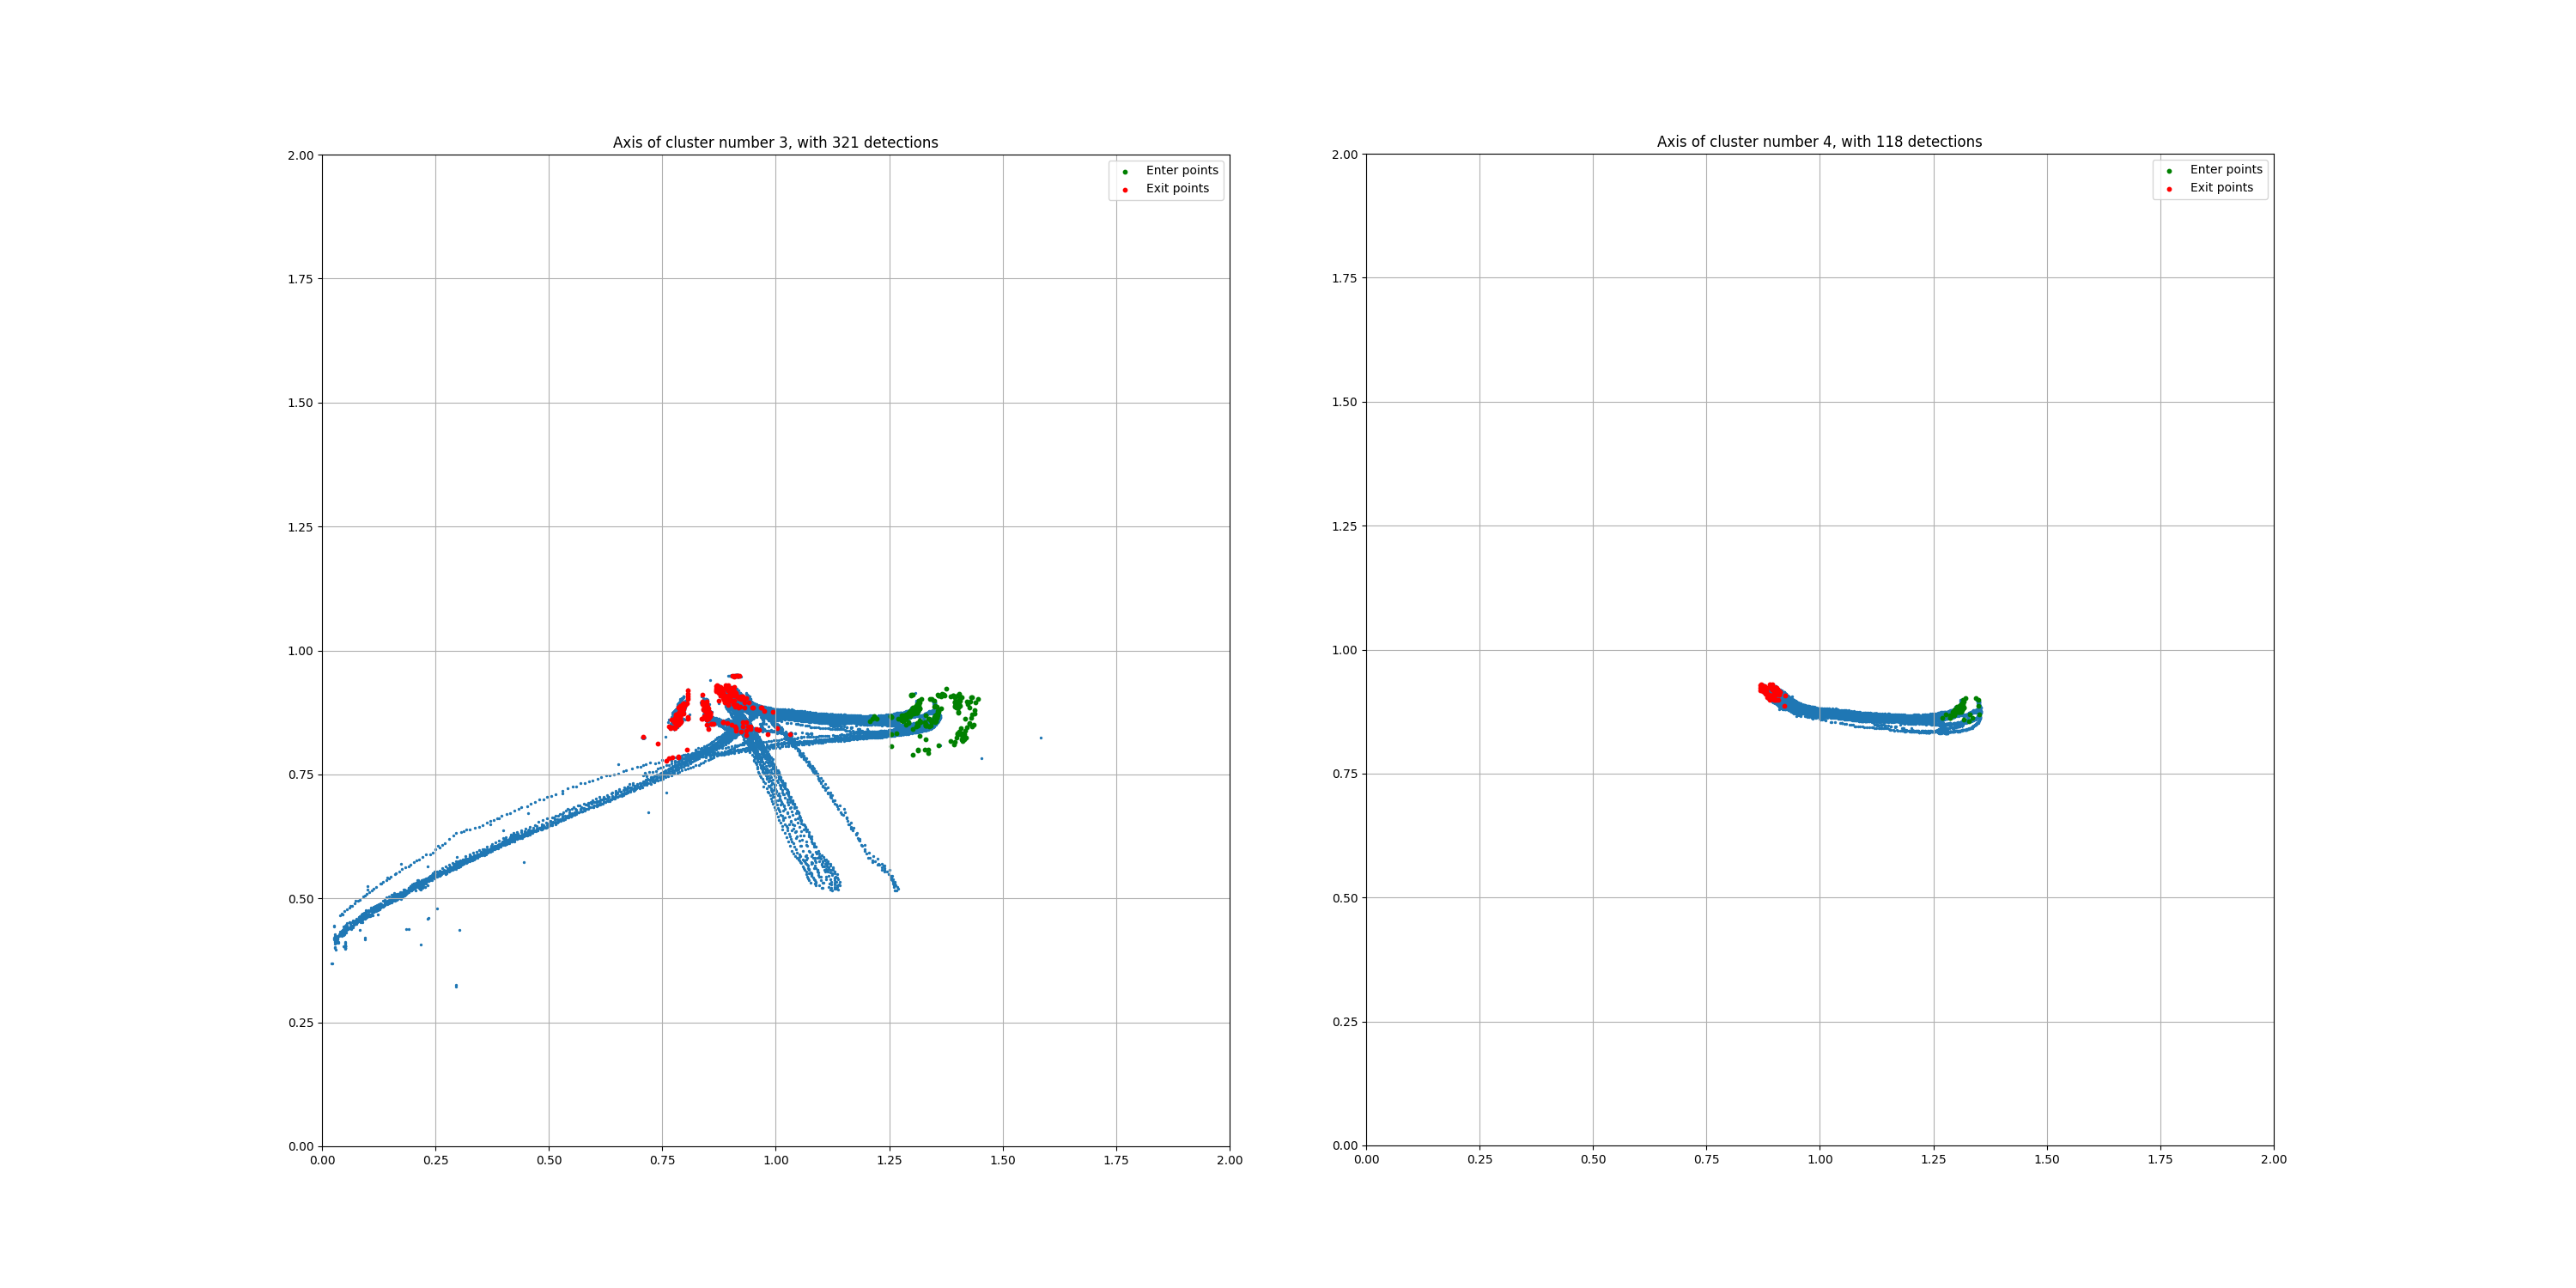
\includegraphics[width=1\columnwidth]{clustering/n_cluster_3_before_after.png}

 \Description{Klaszter 4 szűrés előtt és után}
 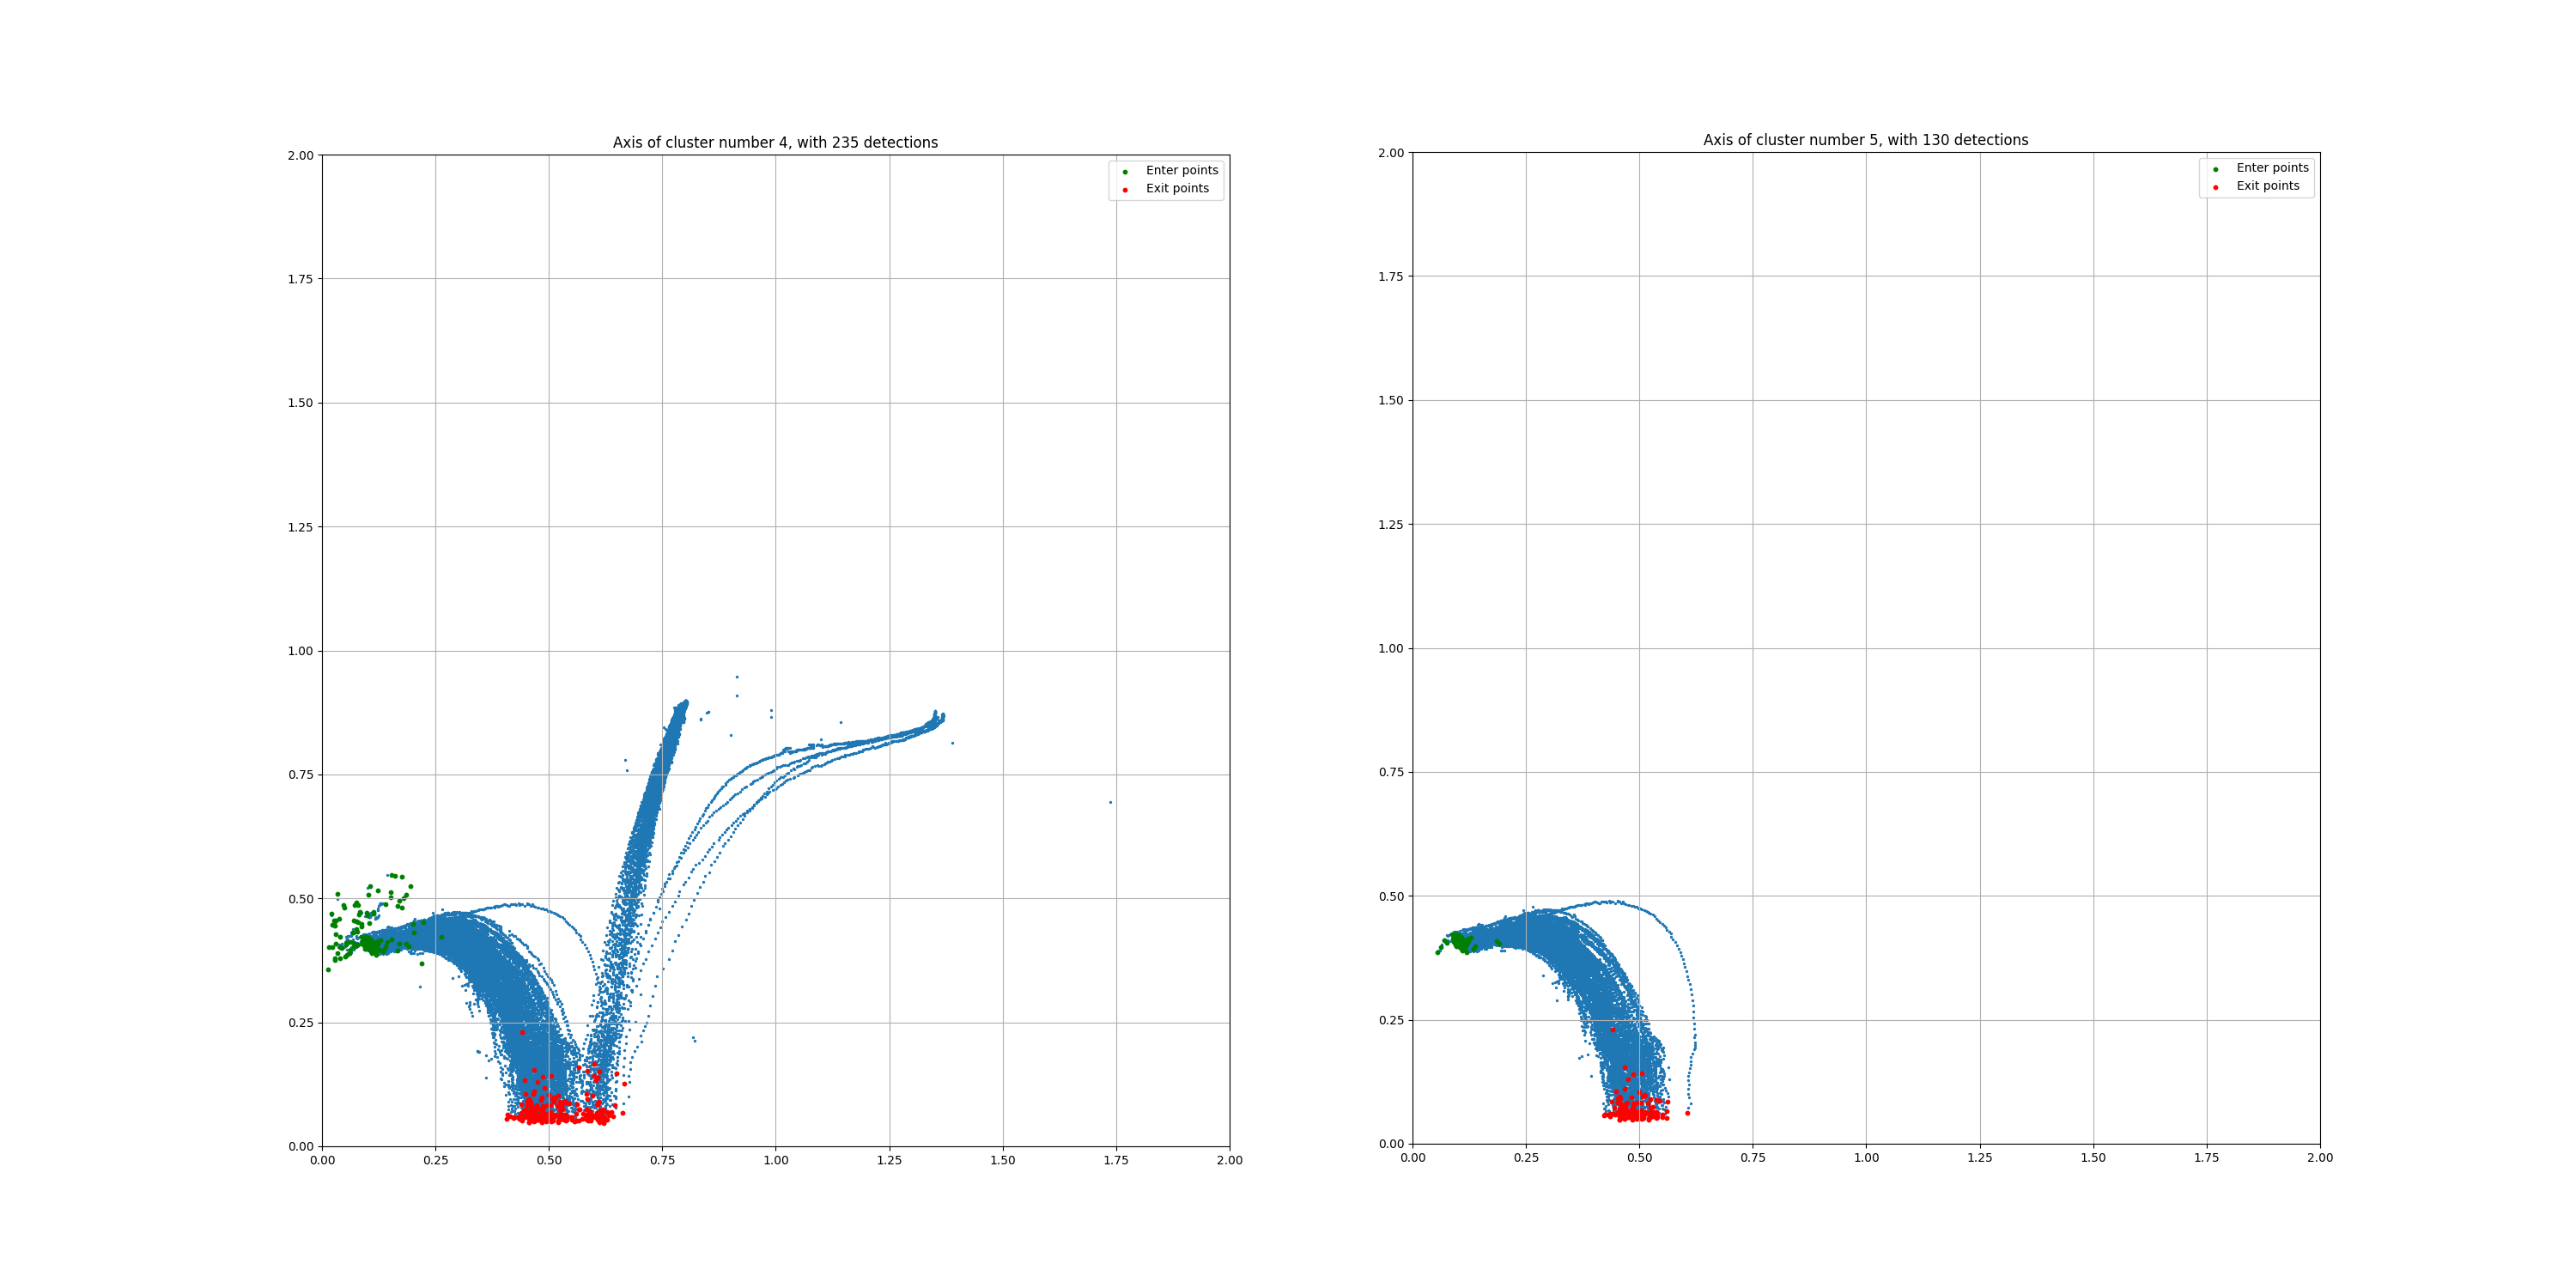
\includegraphics[width=1\columnwidth]{clustering/n_cluster_4_before_after.png}

 \Description{Klaszter 5 szűrés előtt és után}
 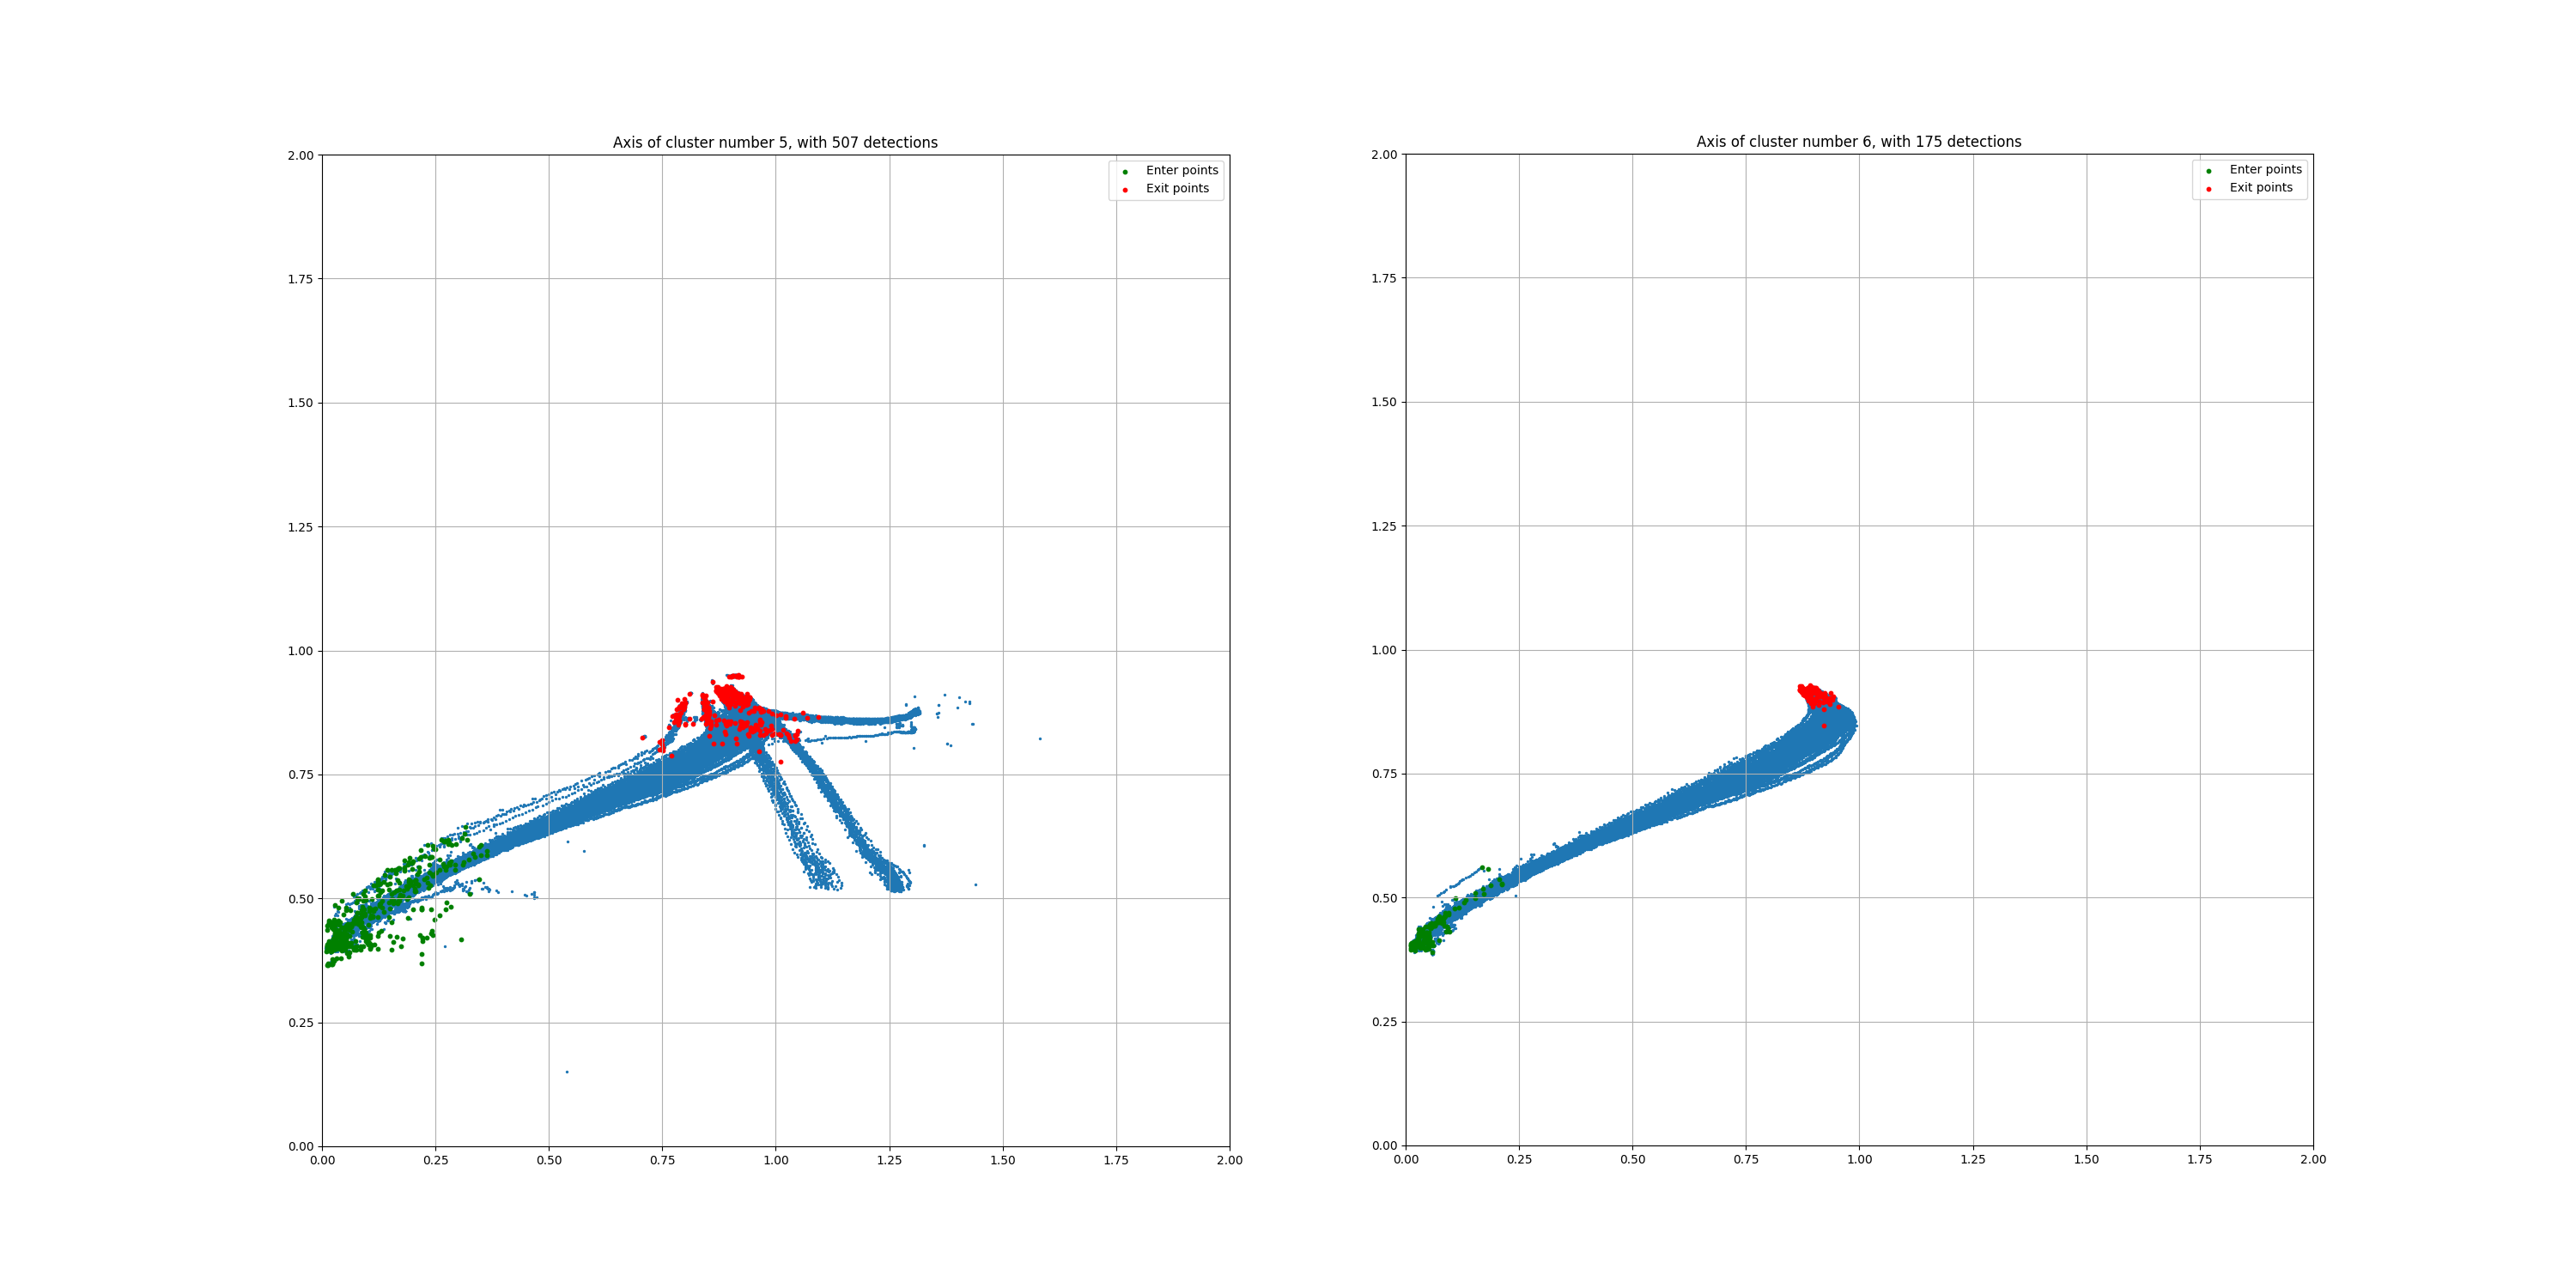
\includegraphics[width=1\columnwidth]{clustering/n_cluster_5_before_after.png}

 \caption{Klaszterezés szűrő}

 \label{fig: Klaszterezés szűrő}   
\end{figure}

\begin{figure}
 \Description{Klaszter 7 szűrés előtt és után}
 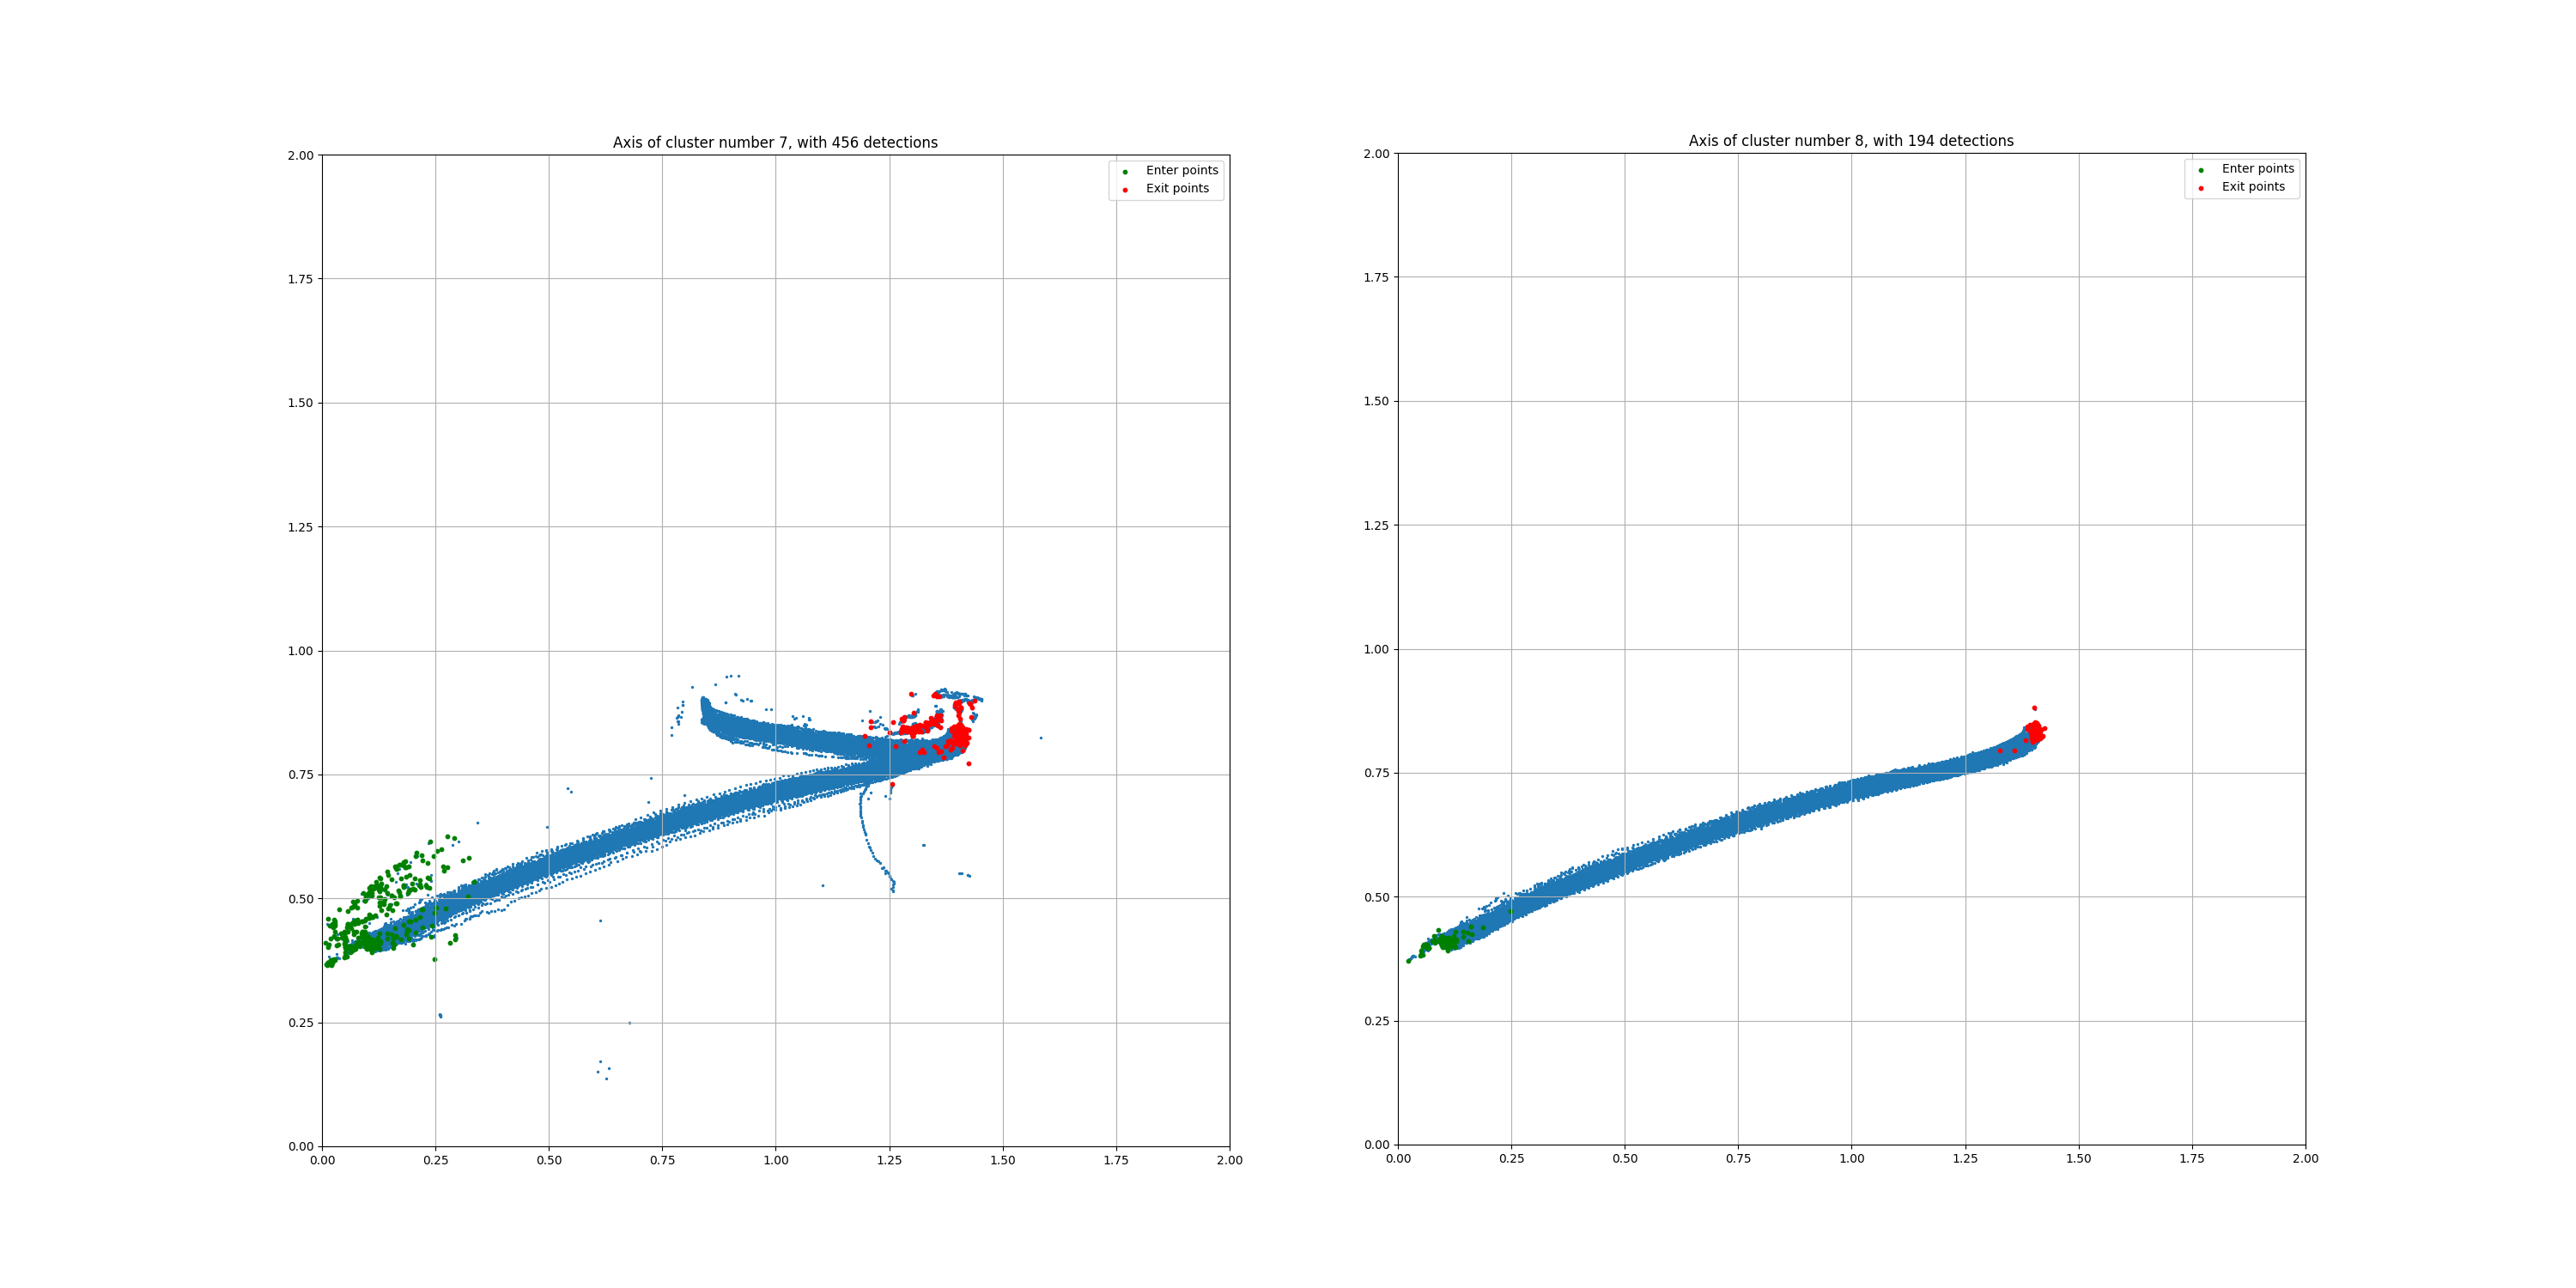
\includegraphics[width=1\columnwidth]{clustering/n_cluster_7_before_after.png}

 \Description{Klaszter 8 szűrés előtt és után}
 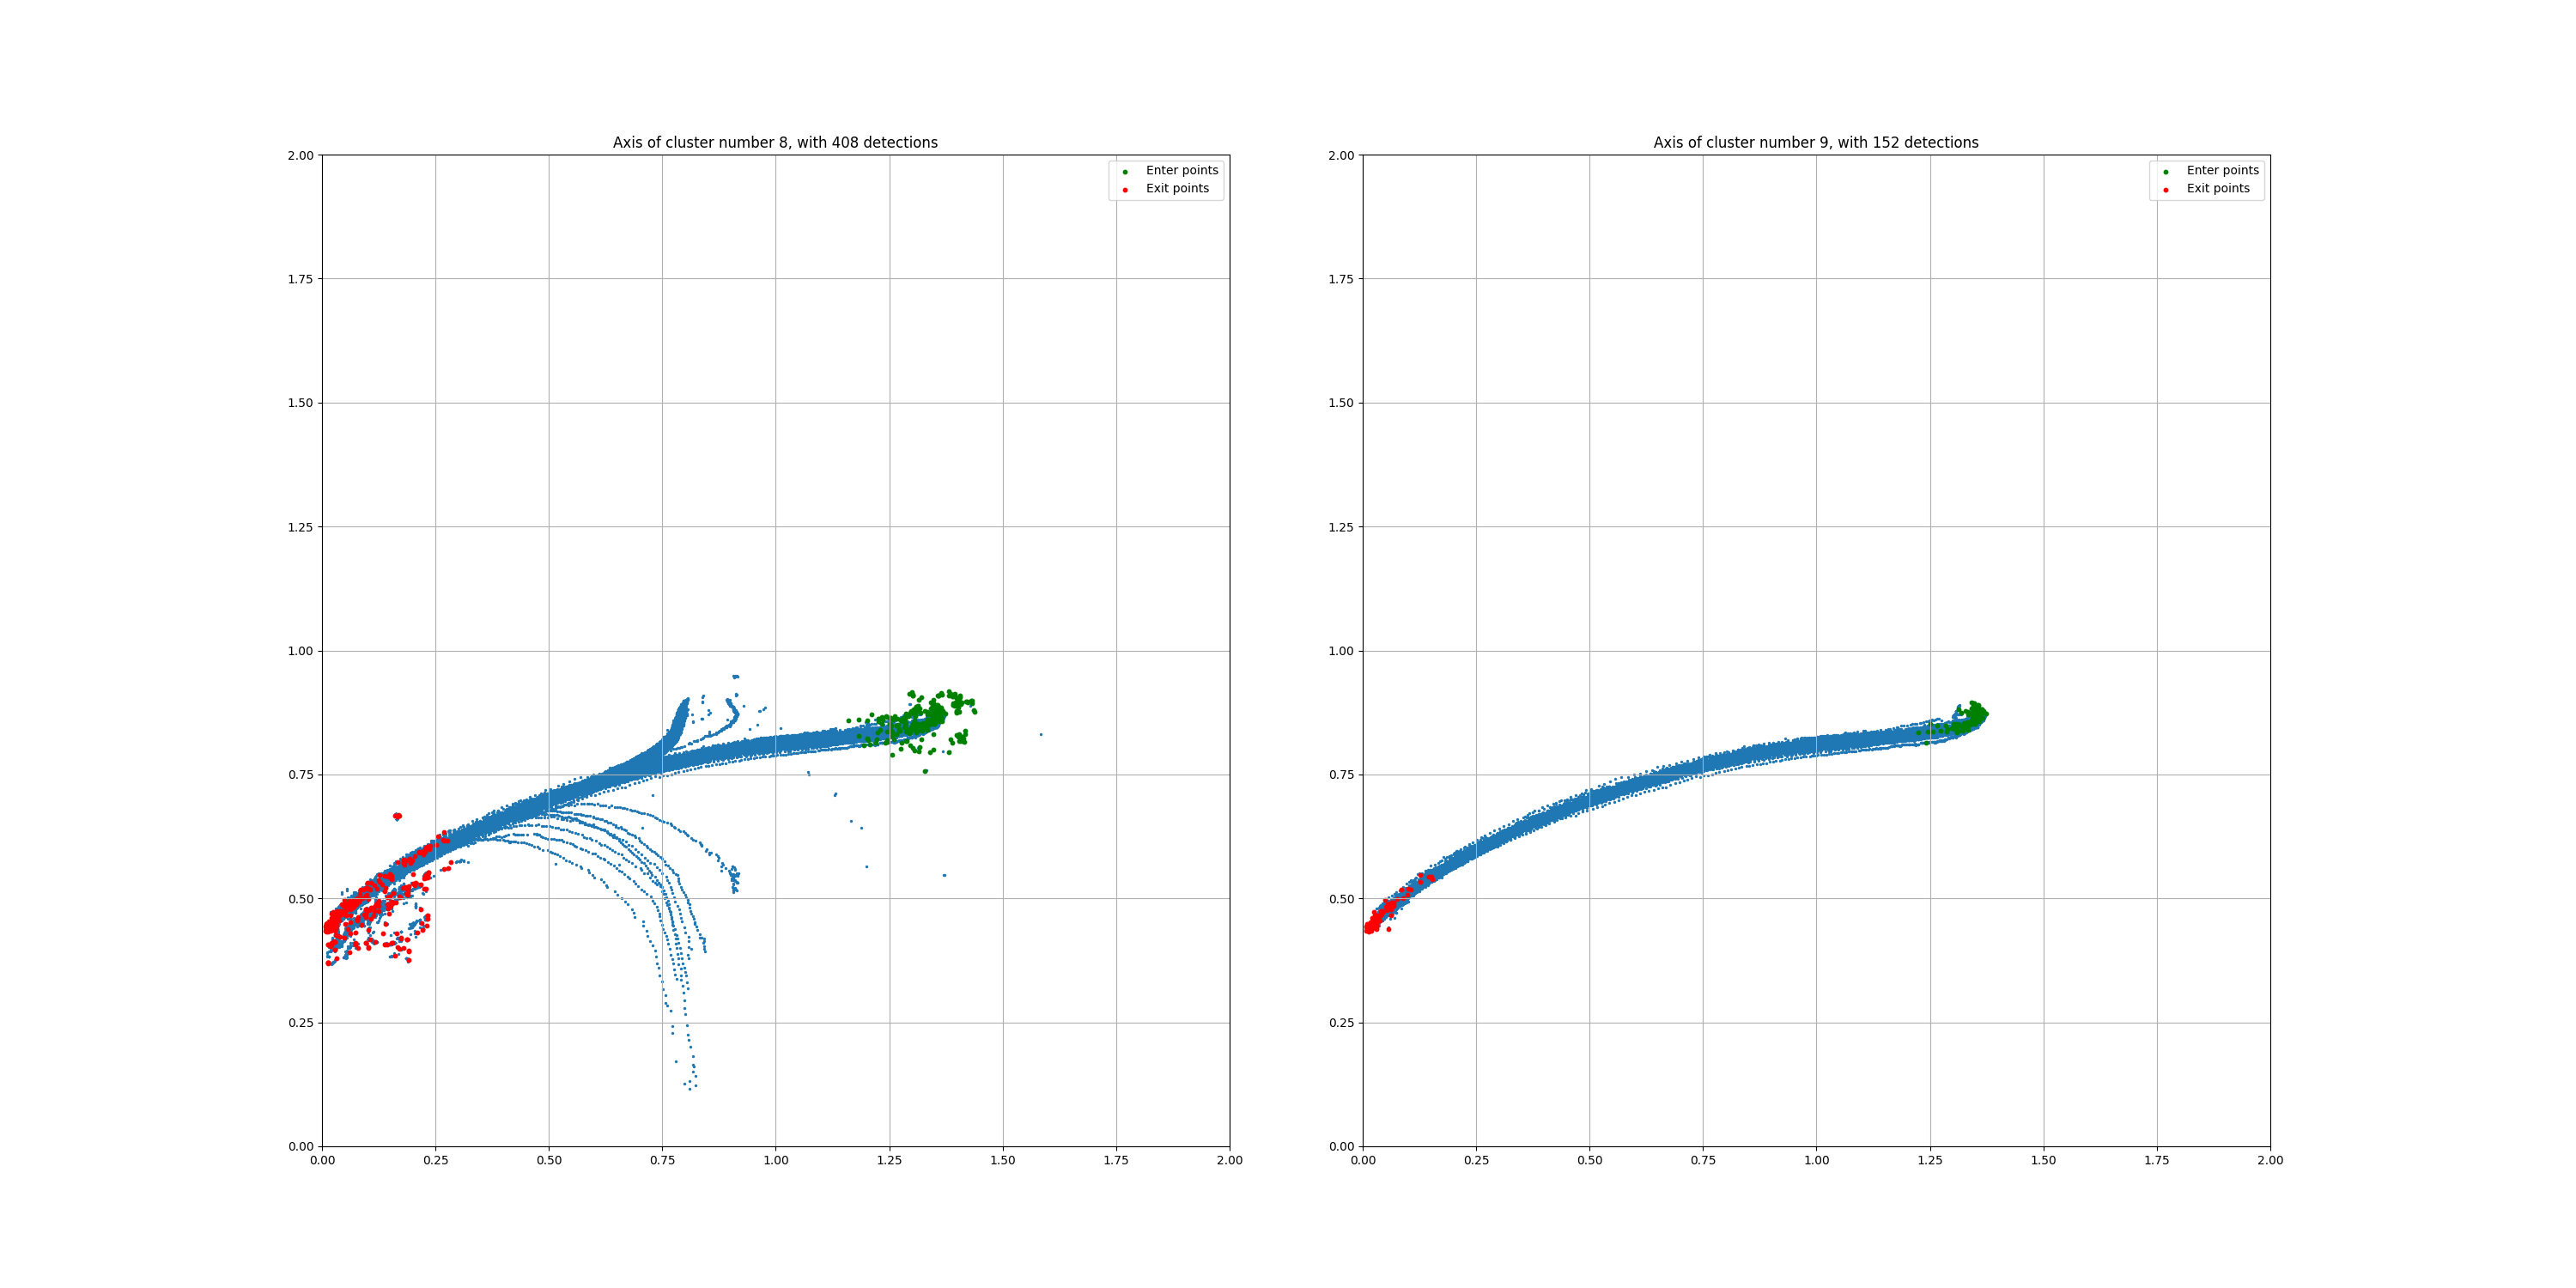
\includegraphics[width=1\columnwidth]{clustering/n_cluster_8_before_after.png}

 \caption{Klaszterezés szűrő }

 \label{fig: Klaszterezés szűrő 2}   
\end{figure}
\subsection{Feature vektorok}
Klaszterezéshez 4 és 6 dimenziós feature vektorokat használ-tunk. A 6 dimenziós vektorokat a DeepSORT hibájának a kiszűrésére hoztuk
létre, felépítésük a következő [belépő x,y középső x,y kilépő x,y], de a kifejlesztett szűrő hatékonyab-bnak bizonyult, és a kevesebb dimenzió is előnyt jelent,
ezért maradtunk a 4 dimenziós feature vektor mellett, aminek a felépítése: [belépő x,y kilépő x,y].
\subsection{Klaszterezési algoritmusok}
Klaszterezéshez több fajta algoritmust teszteltünk. A legjobb eredményeket az OPTICS (Ordering Points To Identify the Clustering Structure) \cite{10.1145/304181.304187} algoritmus adta. 
Aminek az eredményei fenti képeken látható (lásd. \ref{fig: Klaszterezés szűrő}).
OPTICS-on kívül leteszteltük a KMeans, DBSCAN és BIRCH algoritmusokat. KMeans algoritmus egyenlő varianciájú csoportokba osztja a mintákat úgy,
hogy az \begin{math}inercia\end{math} kritériumot csökkentse. A KMeans egy fontos paramétere a \begin{math}n_clusters\end{math}, amivel a várható
klaszterek számát kell megadni. Ennek a paraméternek a meghatározására próbálkoztunk különböző metrikákat felhasználni, hogy automatizálható legyen
a klaszterezési lépés. Ezek a metrikák a Silhouette Coefficient \cite{ROUSSEEUW198753}, Calinski-Harabasz Index \cite{article} és Davies-Bouldin Index \cite{4766909}.
Elbow diagramok segítségével próbáltuk eldönteni, hogy milyen értéket érdemes adni az \begin{math}n_clusters\end{math} paraméternek lásd \ref{fig: Elbow diagramok}.
A mérőszámok konzisztensen alacsony értéket adtak, egy négy ágú kereszteződésnél, ahol jóval több klaszterbe sorolhatók a trajektóriák. A KMeans használatát
ezért elvetettük.

\begin{figure}
    \Description{Elbow Calinski}
    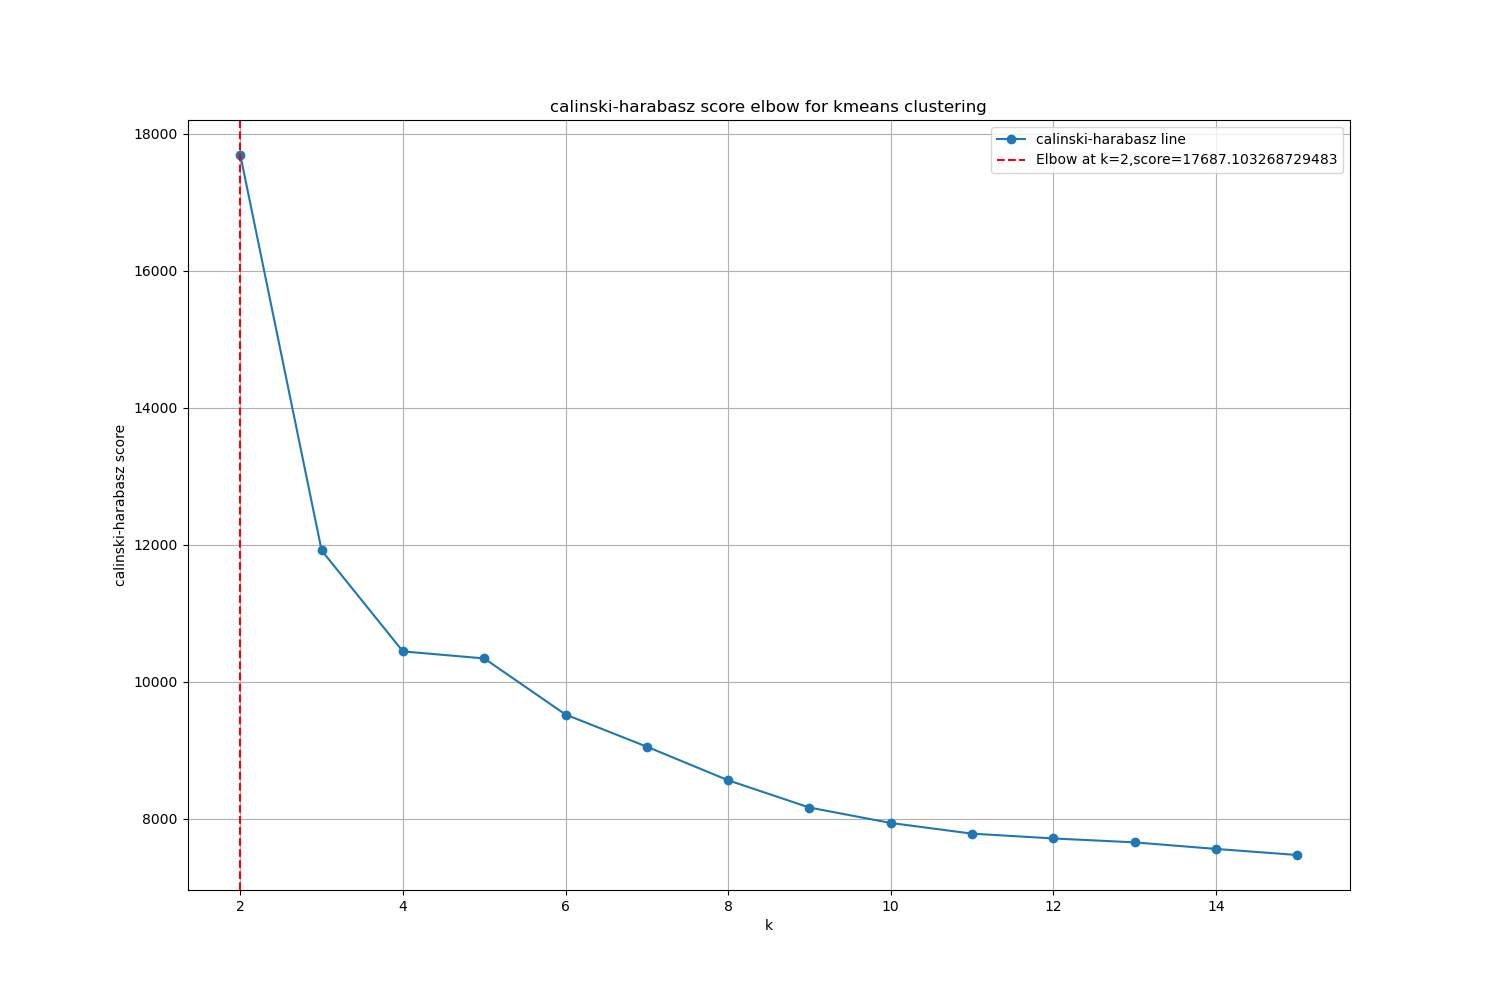
\includegraphics[width=1\columnwidth]{elbow/elbow_on_kmeans_2-16_metric_calinski-harabasz_thresh_0.5.png}

    \Description{Silhouette}
    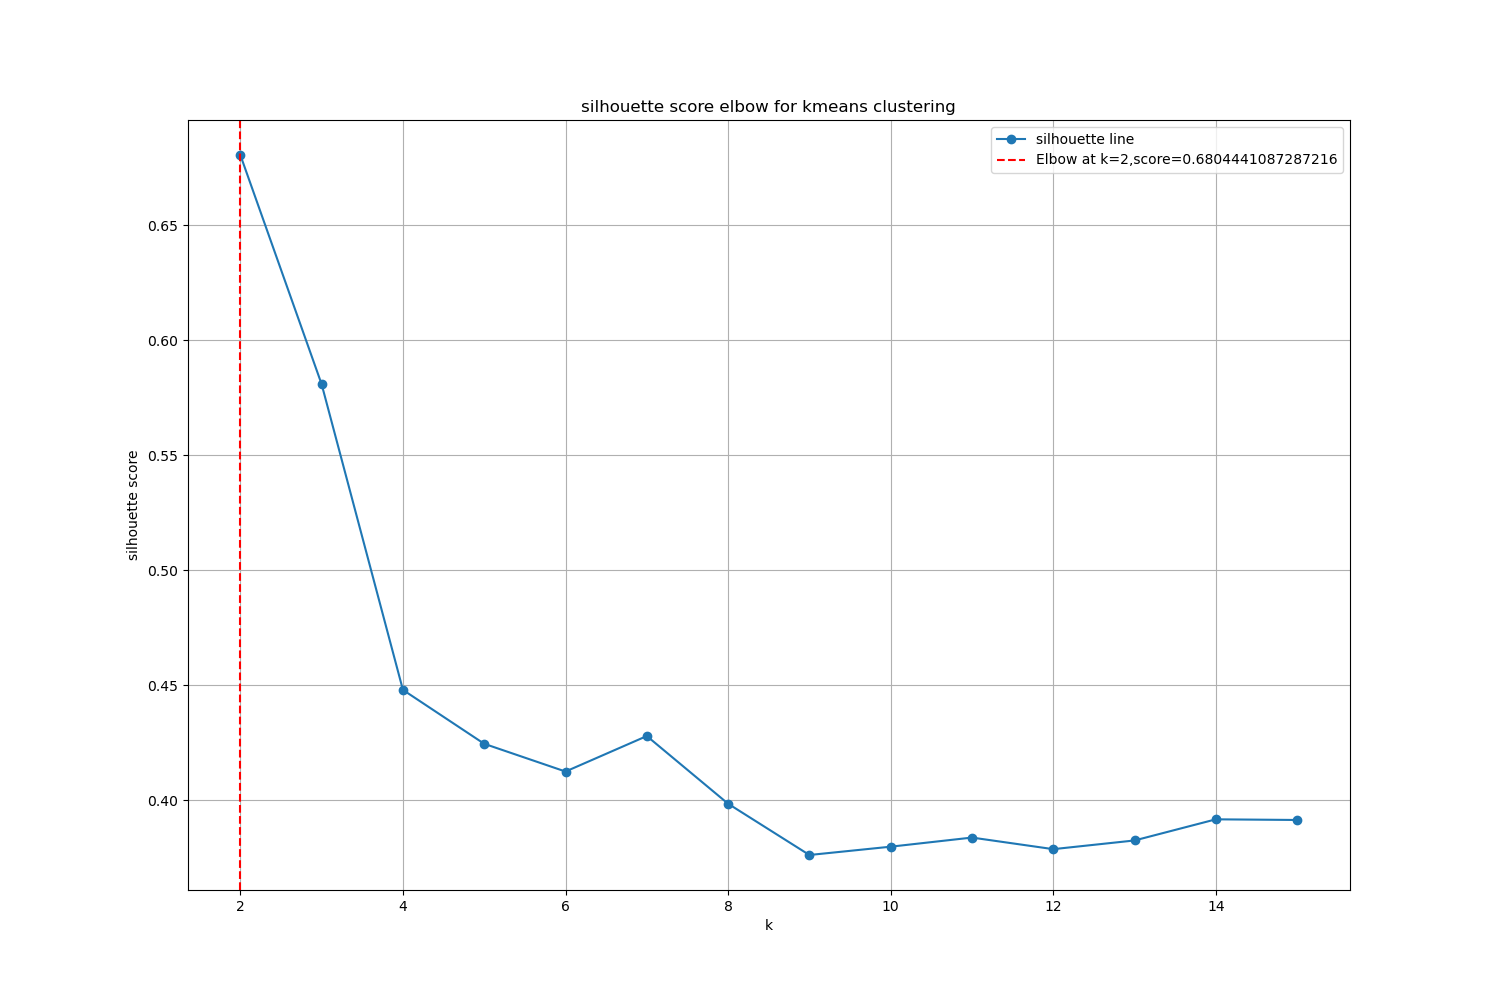
\includegraphics[width=1\columnwidth]{elbow/elbow_on_kmeans_2-16_metric_silhouette_thresh_0.5.png}

    \Description{Davies Bouldin Index}
    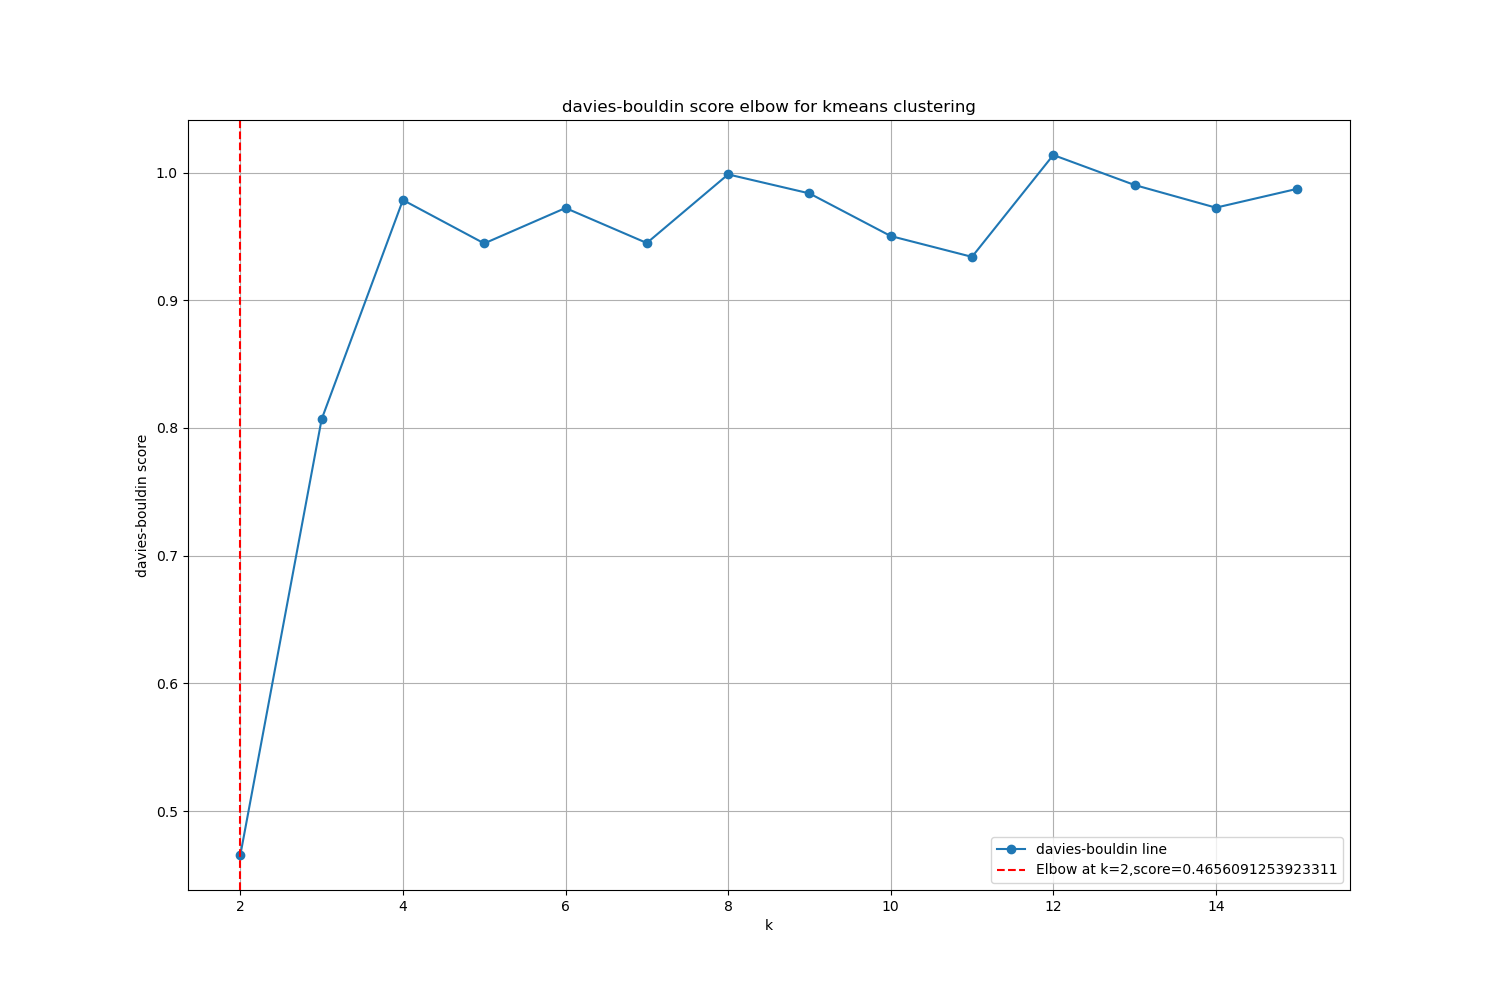
\includegraphics[width=1\columnwidth]{elbow/elbow_on_kmeans_2-16_metric_davies-bouldin_thresh_0.5.png}
    
    \caption{Elbow diagramok}
    \label{fig: Elbow diagramok}
\end{figure}

\begin{figure}
    \Description{KMEans}
    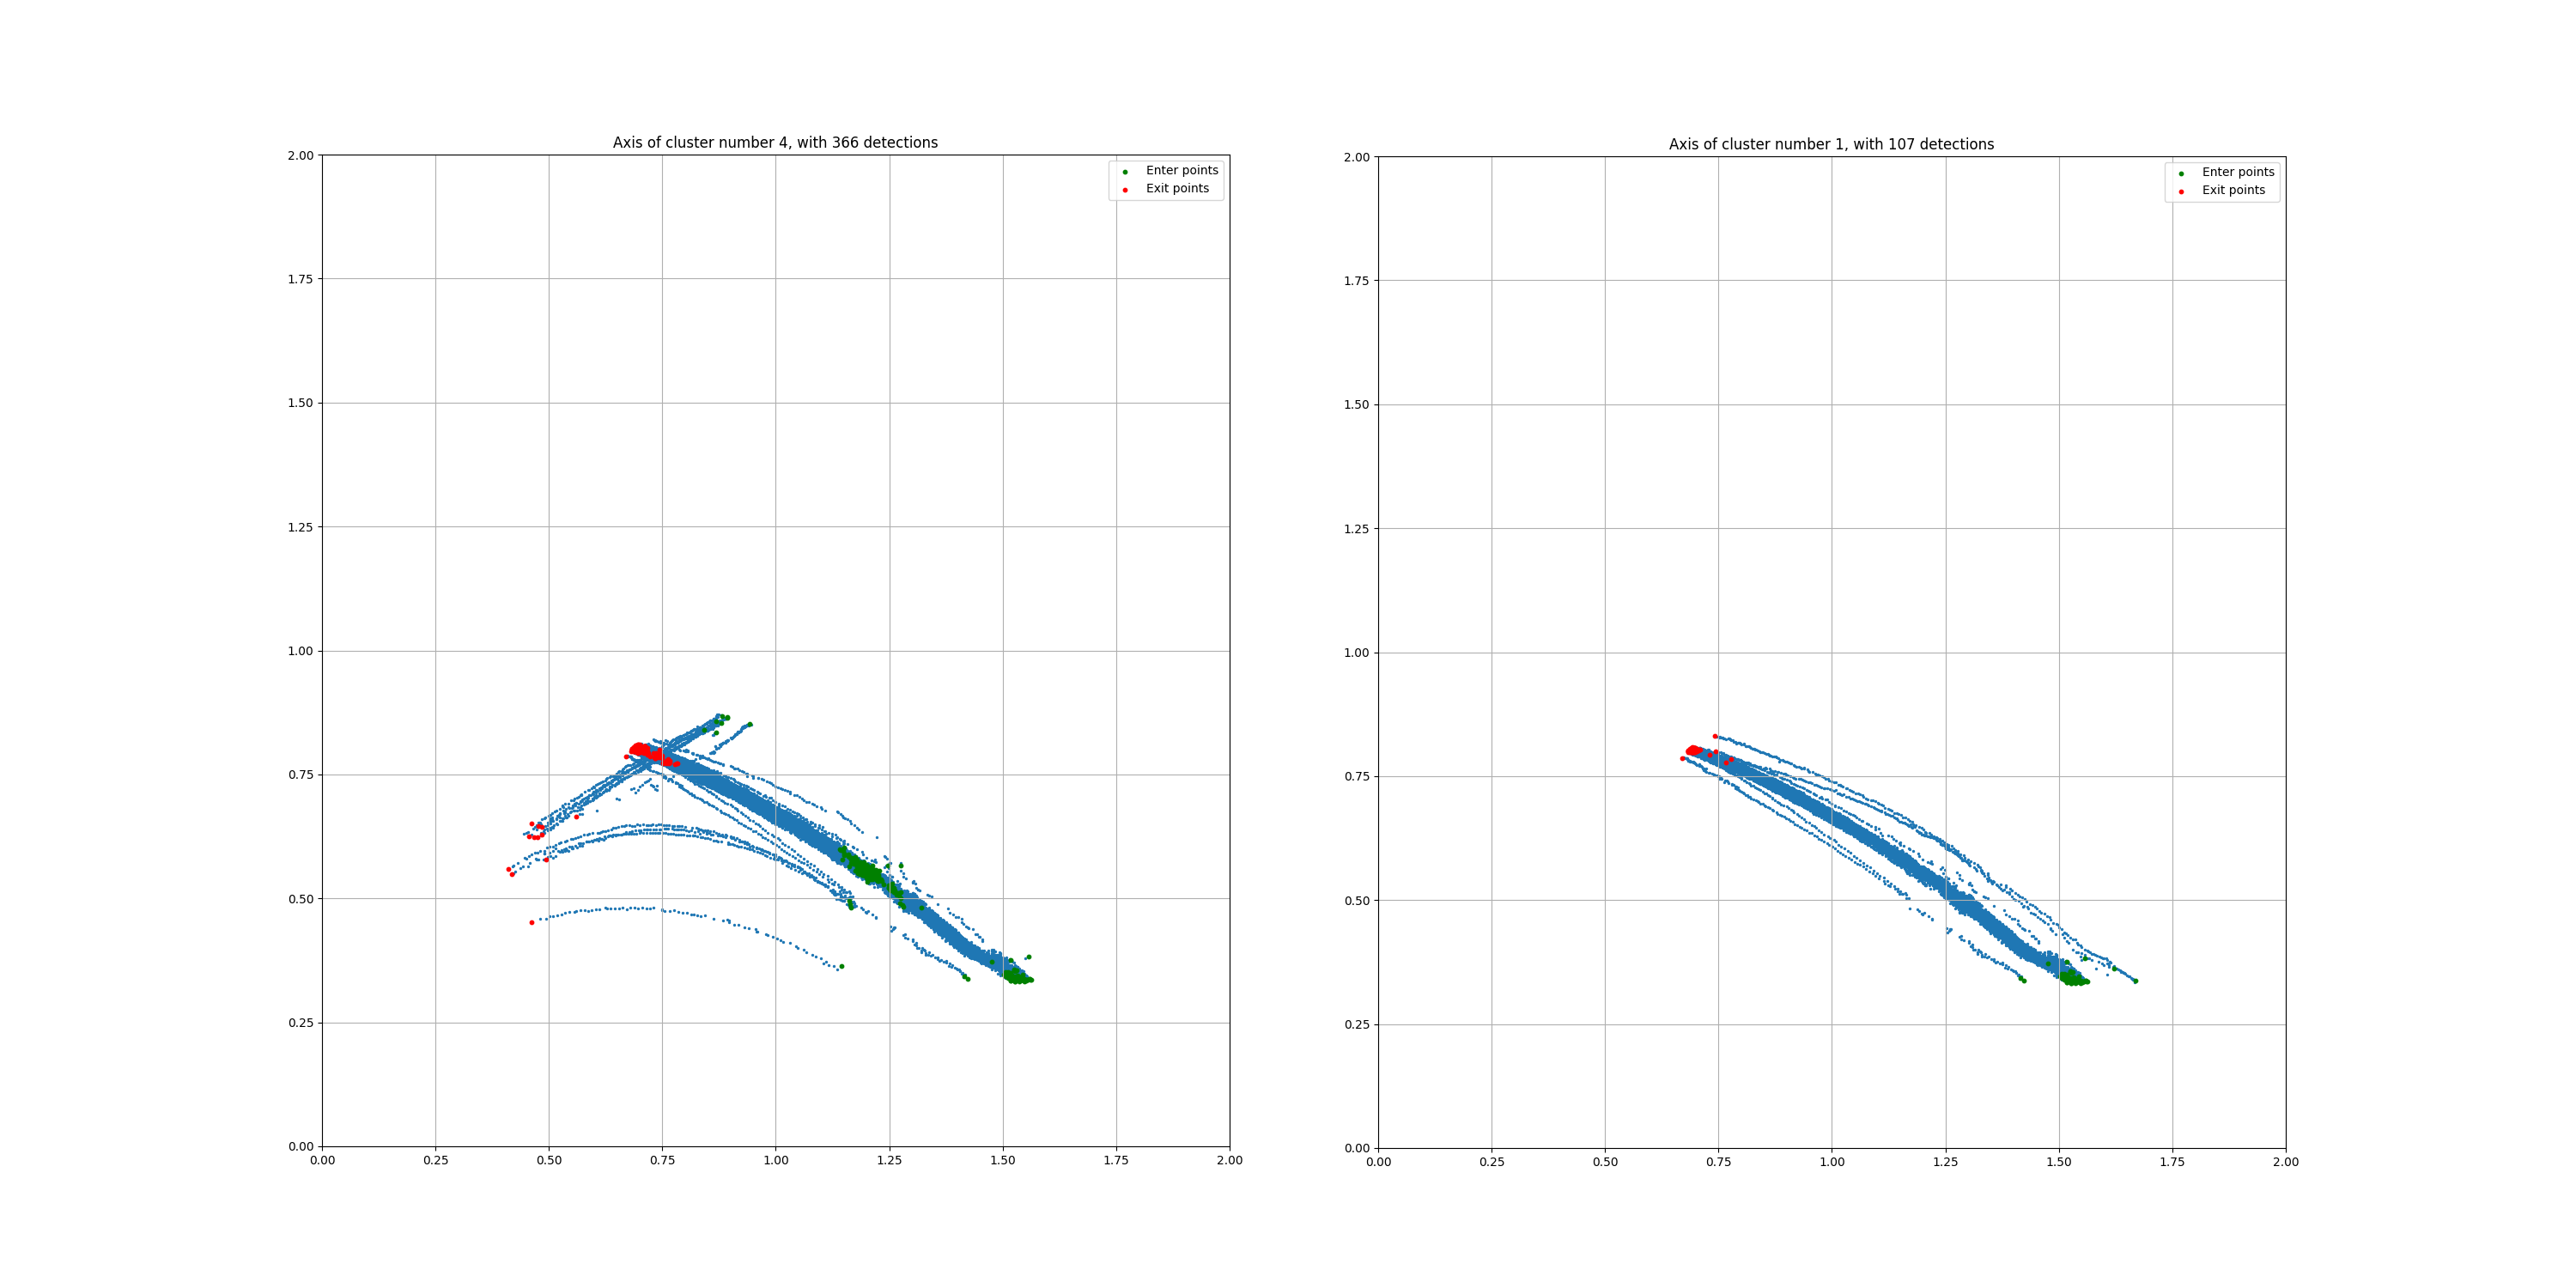
\includegraphics[width=1\columnwidth]{bad_clustering/example_kmeans_vs_optics.png}

    \Description{BIRCH}
    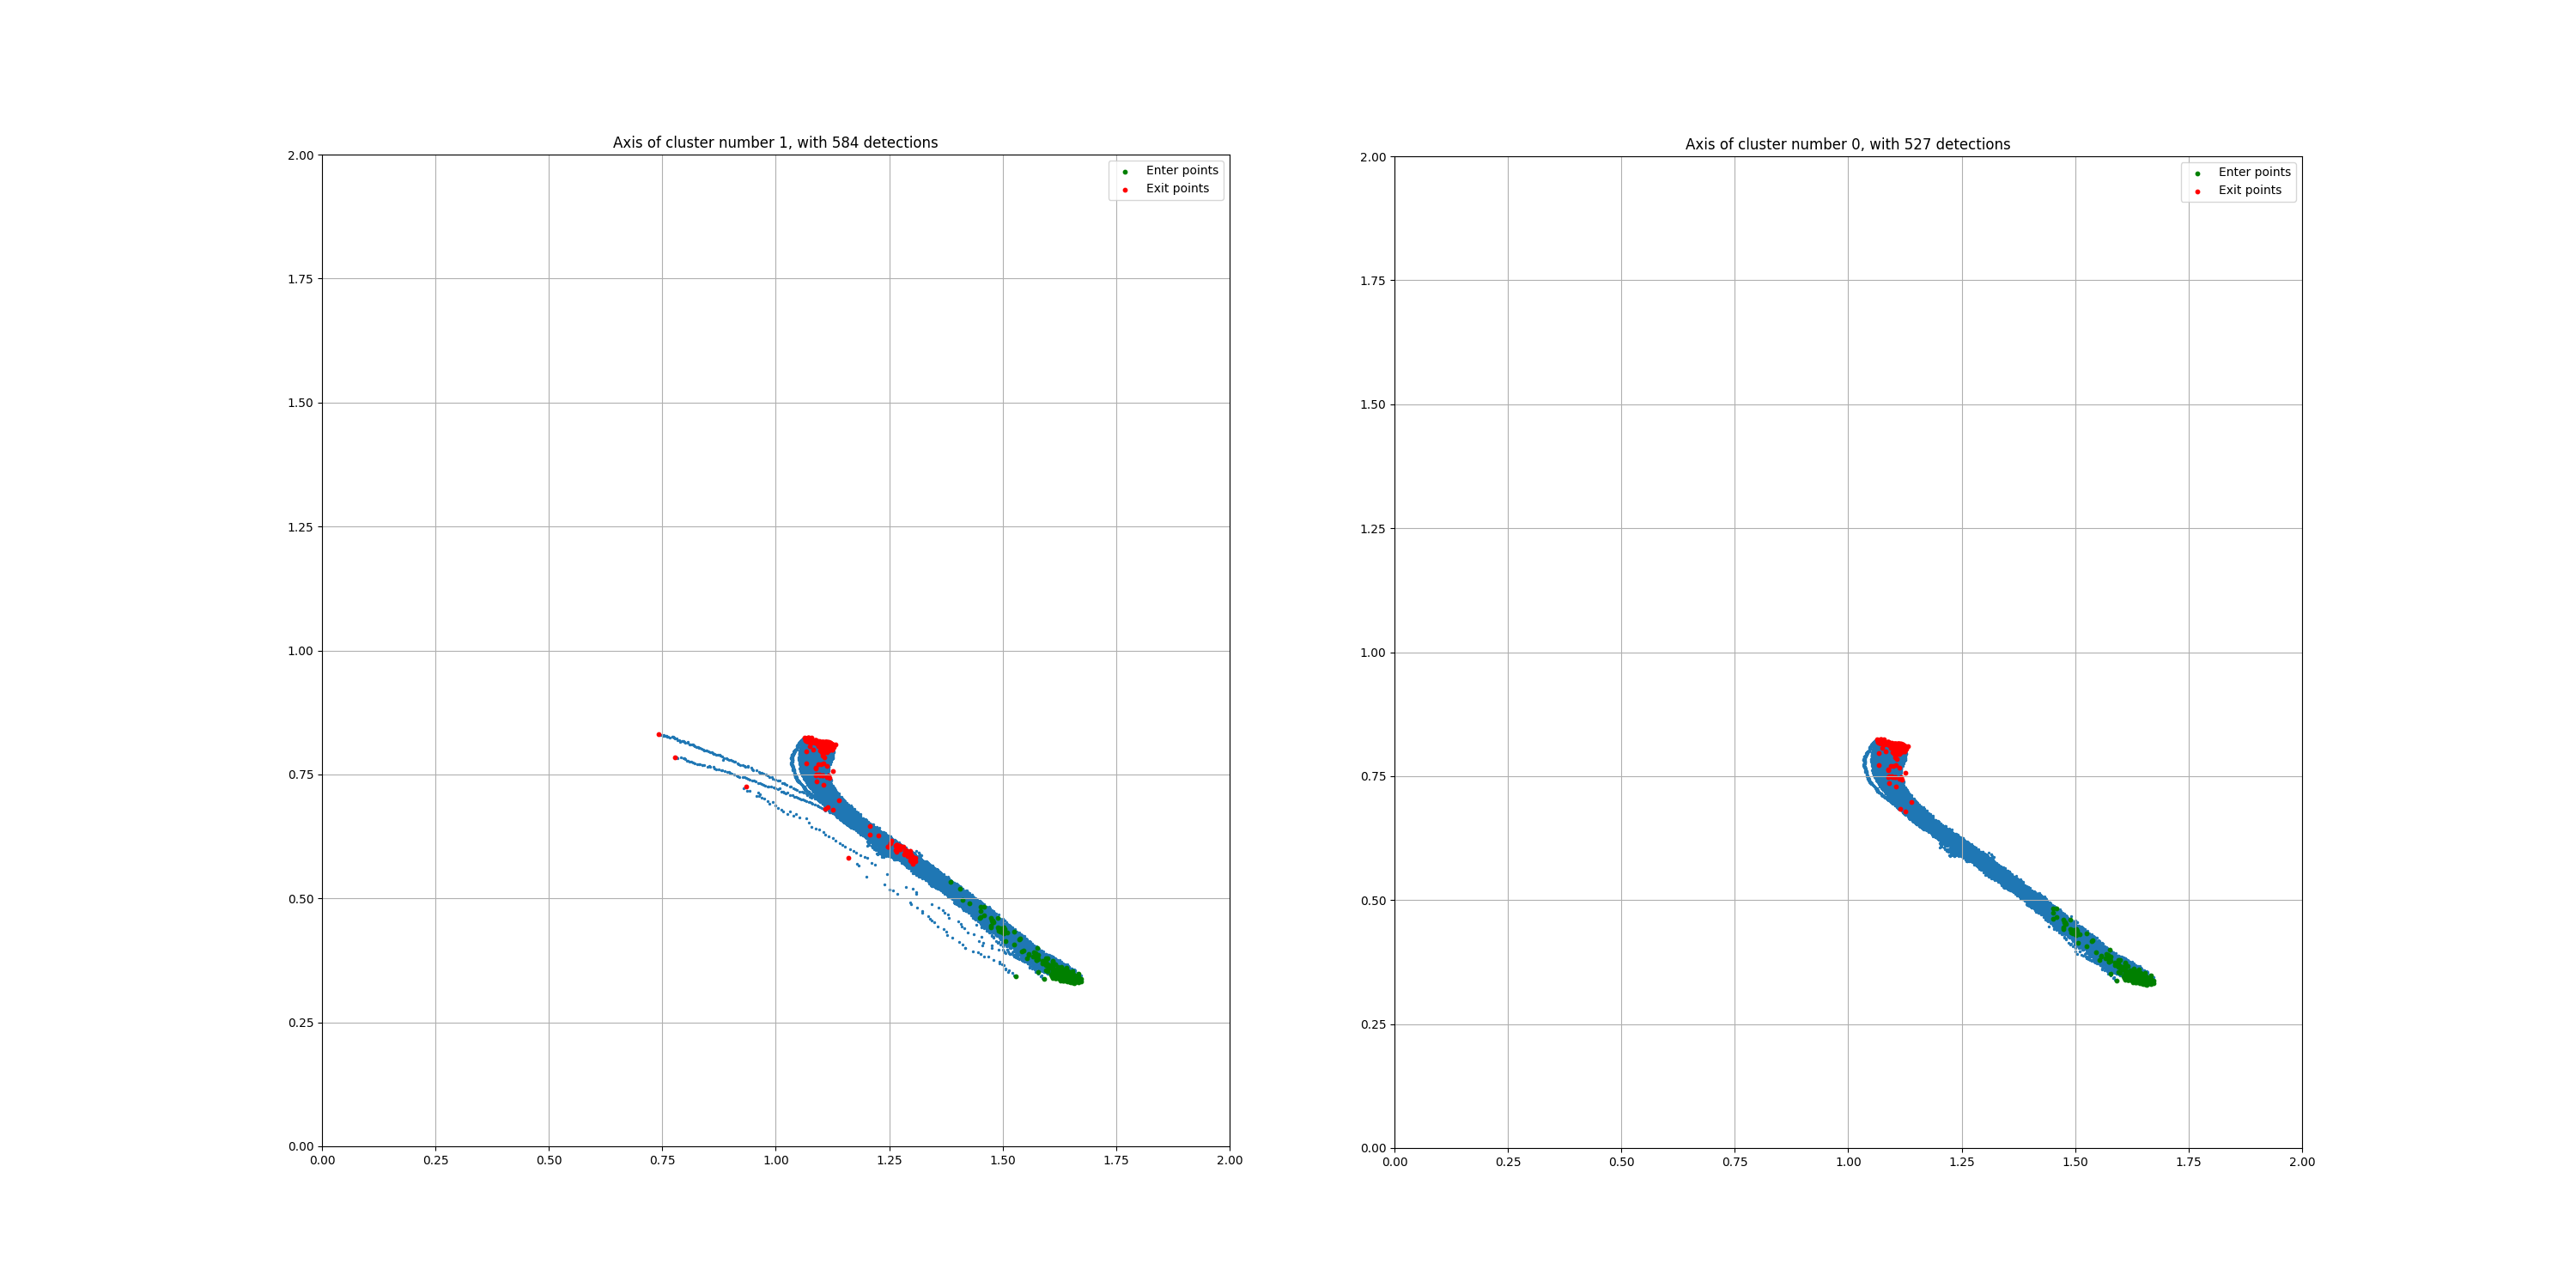
\includegraphics[width=1\columnwidth]{bad_clustering/example_birch_vs_optics.png}

    \Description{DBSCAN vs OPTICS merged cluster}
    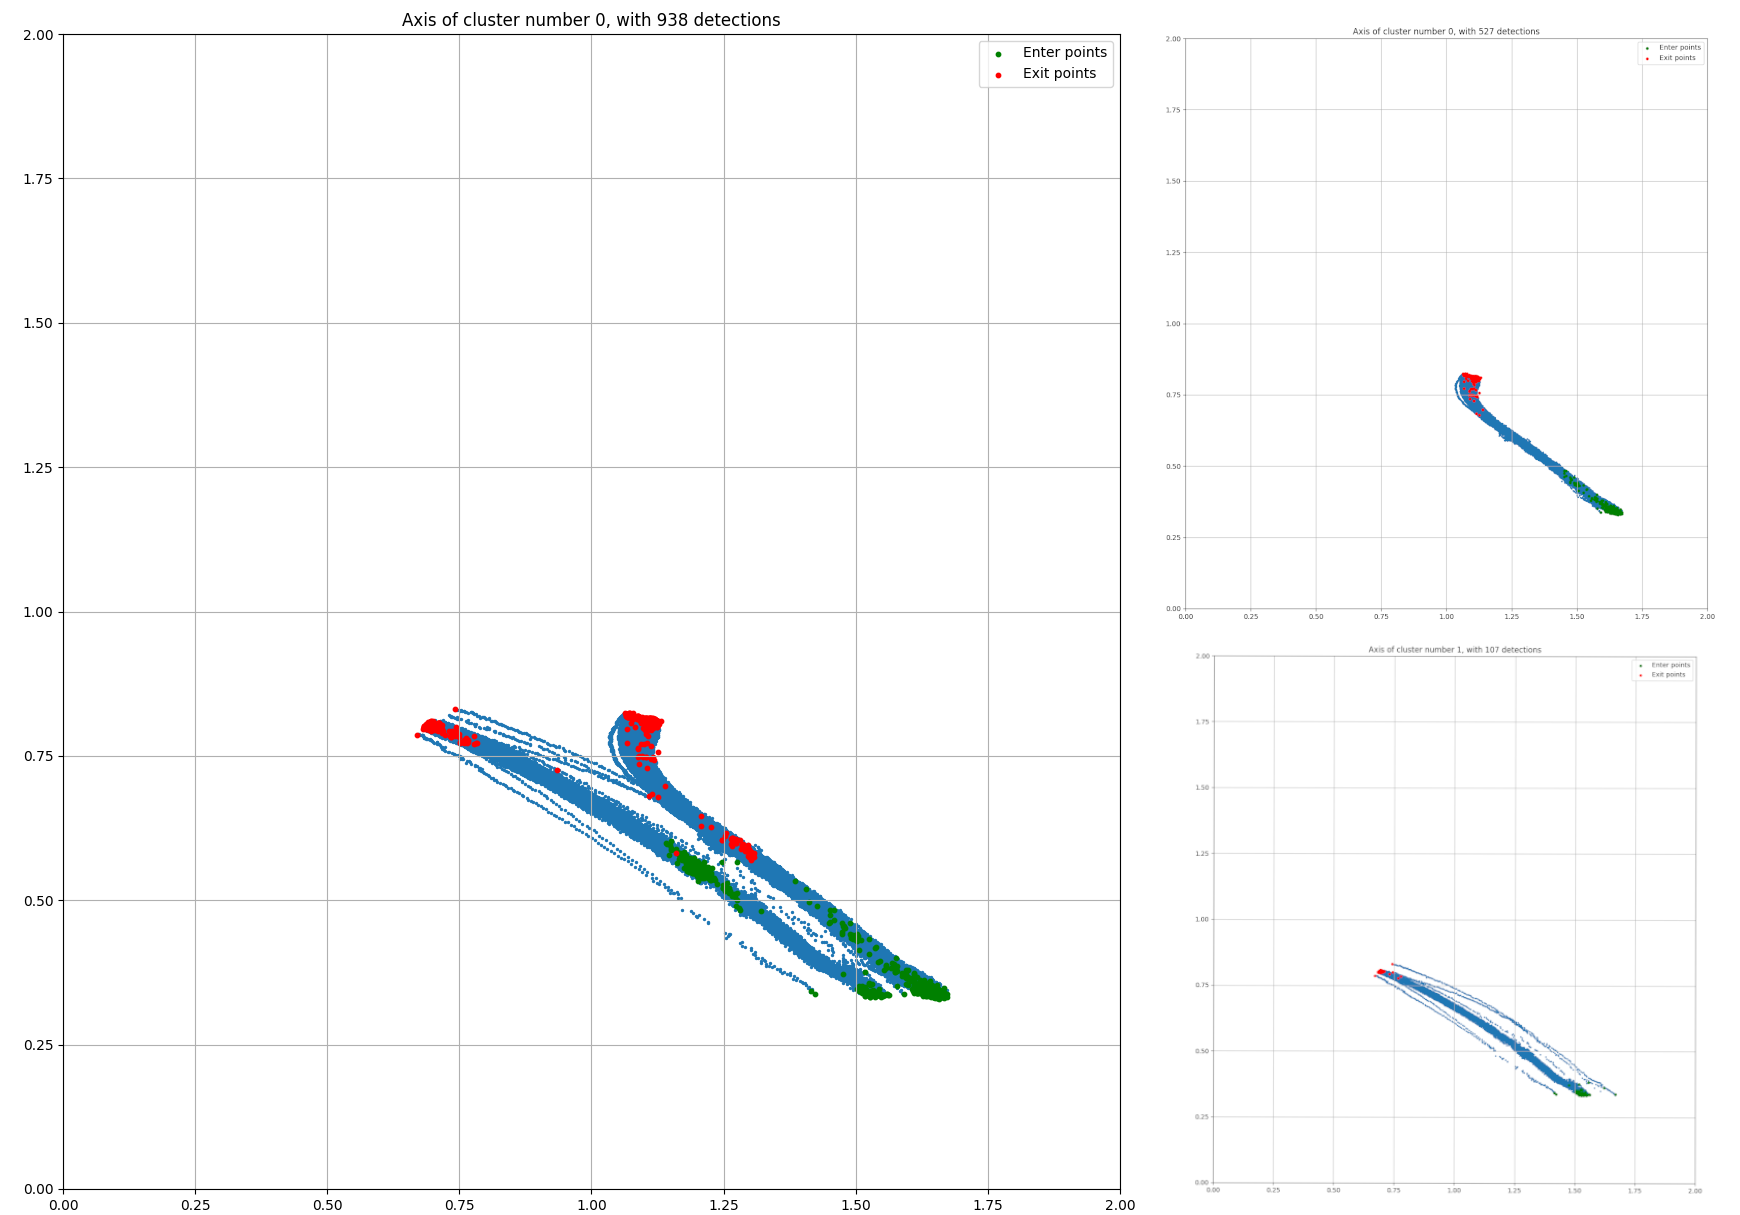
\includegraphics[width=1\columnwidth]{bad_clustering/example_dbscan_vs_optics_merged_cluster.png}

    \caption{KMeans, BIRCH, DBSCAN vs OPTICS}
    \label{fig: Bad clusters}
\end{figure}

A BIRCH algoritmus sokszor egybevon klaszter bemeneteket vagy kimeneteket, ami miatt több más irányból jövő, vagy több más irányba kilépő objektumokat sorol azonos klaszterekbe.
\begin{math}threshold\end{math} paraméterrel lehet a klaszterek méretét szabályozni, amivel javítható az egybevont klaszterek száma, a kutatás során futtatott tesztek alapján, még
így is az OPTICS adta a legtisztább klasztereket. 
DBSCAN algoritmus sokban hasonlít az OPTICS-hoz. A \begin{math}max\_eps\end{math} paraméter helyett, ami egy távolság tartományt ad meg, az \begin{math}eps\end{math} paraméter  
pontos távolságot adja meg, hogy két minta egymás szomszédságában van-e vagy sem, ez egy éles határ, ezért az OPTICS könnyebben finomhangolható.

\subsection{Paraméterek kiválasztása}
A megfelelő paraméterek kiválasztása a klaszterezéshez igen fonzosnak bizonyult. Ezt a gyűjtött adathalmazokon kézzel kellett finomhangolnunk.
A halmazok minimum számosságát a \begin{math}min\_samples\end{math} paraméterrel lehet szabályozni, a pontok egymástól való távolságának
felső határát \begin{math}max\_eps\end{math}-el lehet megadni. Az távolság kiszámítására használt methódust \begin{math}metric\end{math}-el
lehet megadni. A \begin{math}xi\end{math} paraméterrel az elérési plot minimum meredekségét lehet megadni. ami a klaszterek határát szabja meg.
Az adathalmazra alkalmazható megfelelő paramétereket nem tudtuk generalizálni, kézzel kellett finomhangolnunk. A plotokon látható klaszterek
megtalálásához \begin{math}min\_samples=50\end{math}, \begin{math}max\_eps=0.1\end{math}, \begin{math}metric='minkowski'\end{math} és \begin{math}xi=0.15\end{math}
paramétereket használtunk.
\section{Klasszifikáció}
\subsection{Multiclass}
A több osztályos klasszifikálás egy olyan feladat, amikor több mint 2 osztály van, és minden feature vektor csak egy osztályba tartozhat.
Ez kevesebb osztály számnál jó eredeményt adhat, de a mi esetünkben ahol 10-15 osztály is lehet, ami azt jelenti, hogy nem lehet elérni nagy
pontosságot. Ennyi osztály közül nehéz pontosan eltatlálni melyik osztályba tartozik egy trajektória.
\subsection{Binary}
A bináris klasszifikáció a többklasszossal szemben, csak 2 osztály között dönt. 2 osztály között sokkal pontosabban el lehet dönteni,
hogy a feature vektor melyikbe tartozik.
\subsection{OneVsRest}
Binráris klasszifikációs modellek kombinációjából, egy több osztályos modellt állítottunk össze, ami átlagban 90\%-os feletti pontossággal tudta előre
jelezni, hogy mely klaszterbe tartozik a jármű.
\subsection{Machine Learning modellek}
Kutatatásunk során több féle machine learning modellt teszteltünk: KNN (KNearesNeighbors), GNB (GaussianNaiveBayes), MLP (MultiLayerPerceptron), 
SGD (StochasticGradientDescent), SVM/SVC (SupportVectorMachine/SupportVectorClassifier) \cite{CC01a}, DT (DecisionTree) \cite{Breiman1984ClassificationAR}.
Ezekből a GNB, MLP és SGD nem adott jó eredményeket ami látható az alábbi táblázatban \ref{table:1}, az eredmények megismétlődtek későbbi tesztekben, ezért
ezeket a modelleket nem tárgyaljuk. A legjobb eredményeket a KNN adta

\begin{table}[]
\begin{tabular}{|lccc|}
\hline
\multicolumn{4}{|c|}{Feature vektor verzió 1}                                                                     \\ \hline
\hline
\multicolumn{1}{|l|}{Metrics}            & \multicolumn{1}{c|}{Balanced} & \multicolumn{1}{c|}{Top 1}   & Top 2   \\ \hline
\multicolumn{1}{|l|}{KNN}                & \multicolumn{1}{c|}{90.57\%}  & \multicolumn{1}{c|}{95.50\%} & 99.12\% \\ \hline
\multicolumn{1}{|l|}{GNB}                & \multicolumn{1}{c|}{63.92\%}  & \multicolumn{1}{c|}{73.25\%} & 90.10\% \\ \hline
\multicolumn{1}{|l|}{MLP}                & \multicolumn{1}{c|}{58.49\%}  & \multicolumn{1}{c|}{81.93\%} & 89.43\% \\ \hline
\multicolumn{1}{|l|}{SGD Modified Huber} & \multicolumn{1}{c|}{45.43\%}  & \multicolumn{1}{c|}{66.39\%} & 83.54\% \\ \hline
\multicolumn{1}{|l|}{SGD Log Loss}       & \multicolumn{1}{c|}{40.41\%}  & \multicolumn{1}{c|}{60.70\%} & 79.69\% \\ \hline
\multicolumn{1}{|l|}{SVM}                & \multicolumn{1}{c|}{77.87\%}  & \multicolumn{1}{c|}{89.29\%} & 96.61\% \\ \hline
\multicolumn{1}{|l|}{DT}                 & \multicolumn{1}{c|}{90.95\%}  & \multicolumn{1}{c|}{93.64\%} & 95.06\% \\ \hline
\end{tabular}
\caption{Feature vektor verzió 1}
\label{table:1}
\end{table}

\begin{table}[]
\begin{center}
\begin{tabular}{|lccc|}
\hline
\multicolumn{4}{|c|}{\begin{tabular}[c]{@{}c@{}}Average Accuracy \\ Feature Vector v1\end{tabular}}    \\ \hline
\hline
\multicolumn{1}{|l|}{Metrics} & \multicolumn{1}{c|}{Balanced} & \multicolumn{1}{c|}{Top 1}   & Top 2   \\ \hline
\multicolumn{1}{|l|}{KNN}     & \multicolumn{1}{c|}{94.22\%}  & \multicolumn{1}{c|}{96.82\%} & 99.51\% \\ \hline
\multicolumn{1}{|l|}{SVM}     & \multicolumn{1}{c|}{81.05\%}  & \multicolumn{1}{c|}{90.69\%} & 98.16\% \\ \hline
\multicolumn{1}{|l|}{DT}      & \multicolumn{1}{c|}{93.83\%}  & \multicolumn{1}{c|}{95.56\%} & 96.65\% \\ \hline
\end{tabular}
\end{center}
\caption{OneVsRest verzió 2 feature vektorok}
\label{table:2}
\end{table}

\subsection{Feature vektorok}
Ahogyan klaszterezésnél is, fontos meghatározni egy olyan feature vektort, ami a legjobban jellemzi a trajektóriát. Ebben a papírban
két fajta vektor verziót fogunk tárgyalni, amik a tesztek során a legjobban teljesítettek. 
\paragraph{Az első verzió} Felépítése a következő \begin{math}[x_0, y_0, v_{x_0}, v_{y_0}, x_m, y_m, x_l, y_l, v_{x_l}, v_{y_l}]\end{math}, ahol \begin{math}m\end{math}
index jelöli az időben középen elhelyezkedő detektálást, az \begin{math}l\end{math} index pedig az utolsó, legfrissebb detektálást jelőli.
Ez a vektor jól reprezentálja a valós idejű futás közben keletkező trajektóriákat, mert egyszerre több száz detektálást objektumonként
nem lehet eltárolni a memórában, hanem egy meghatározott méretű buffert kell alkalmazni, aminek mi 15 vagy 30 detektálást adtunk.
Az adathalmazban eltárolt trajektóriák ennél a buffernél több detektálást tartalmaznak, ezért az első verziónál a trajektóriát \begin{math}k\end{math} 
részre osztottuk, így egy trajektória szelet mérete \begin{math}s_n = n_d/k\end{math}, ahol \begin{math}n_d\end{math} a detektálások számossága
a trajektóriában. Ezekből a szeletekből képeztük az egyes feature vektorokat.
\paragraph{A másik verzió} Felépítése \begin{math}[x_0 * w_1, y_0 * w_2, v_{x_0} * w_3, v_{y_0} * w_4, x_l * w_5, y_l * w_6, v_{x_l} * w_7, v_{y_l} * w_8]\end{math}.
Ennél a verziónál használtunk súlyokat, ahol \begin{math}w_1=1\end{math}, \begin{math}w_2=1\end{math}, \begin{math}w_3=100\end{math}, \begin{math}w_4=100\end{math},
\begin{math}w_5=2\end{math}, \begin{math}w_6=2\end{math}, \begin{math}w_7=200\end{math}, \begin{math}w_8=200\end{math}. Mivel a sebességek két 
nagyságrenddel kisebbek mint a koordináták, ezért felszoroztuk őket 100-as súlyokkal. Hogy a 15-30 detektálás nagyságú bufferekben nagyobb hangsúlyt kapjanak a legfrissebb
koordináták és sebességek, így azok 2-es és 200-as szorzót kaptak.
\paragraph{Teszt eredmények} Azt mutatják, hogy az utóbbi verzió magasabb pontosságokat produkált (lásd \ref{}).

\subsubsection{Adatdúsítás}
Hogy minél pontosabban reprezentáljuk a valód idejű futást, a gyűjtött trajektóriákból nem trajektóriánként egy feture vektort
generáltunk. Ezeknek a szá-mosságát a feature vektort felépítő algoritmusban szabtuk meg.
%\subsubsection{Klassz kiegyenlítés}
\subsection{Pontosság mérése}
A pontosság mérésére háromféle metrikát használtunk.
\paragraph{Accuracy Score}
Ha \begin{math}\hat{y_i}\end{math} az \begin{math}i\end{math}. minta predikciója és \begin{math}y_i\end{math} a hozzá-tartozó valódi érték,
akkor az eltalált predikciók és összes predikció hányadosa, amit így lehet leírni:\break
\begin{equation}
\texttt{accuracy}(y, \hat{y}) = \frac{1}{n_\text{samples}} \sum_{i=0}^{n_\text{samples}-1} 1(\hat{y}_i = y_i)
\end{equation}
\paragraph{Balanced Accuracy}
amit ezért használtunk, hogy az adathalmaz kiegyensúlyozatlansága miatt ne kapjunk fals pontosságot. Ha minden osztályra egyenlően jól teljesít a klasszifikációs modellünk, akkor a sima \emph{Accuracy}-t kapjuk vissza.
Ha a teszt adathalmaz kiegyensúlyozatlansága miatt az egyik osztálynak jobb a pontossága mint egy másiknak, akkor ezt az értéket
elosztja a számával. Ha az \begin{math}y_i\end{math} a valódi értéke az \begin{math}i\end{math}. mintának, és
\begin{math}w_i\end{math} a hozzátartozó súly, akkor ezt a súlyt a következőképpen korrigáljuk:
\begin{equation}
    \hat{w}_i = \frac{w_i}{\sum_j{1(y_j = y_i) w_j}}
\end{equation}
ahol \begin{math}1(x)\end{math} a karakterisztikus függvény. Adott a \begin{math}\hat{y_i}\end{math} perdikció az \begin{math}i\end{math}.
mintának, így a balanced accuracy-t így definiálhatjuk:
\begin{equation}
    \texttt{balanced-accuracy}(y, \hat{y}, w) = \frac{1}{\sum{\hat{w}_i}} \sum_i 1(\hat{y}_i = y_i) \hat{w}_i
\end{equation}
\paragraph{Top-K Accuracy}
az \emph{Accuracy Score} egy generalizált változa-ta. A különbség az, hogy a predikció akkor számít igaznak, ha beletartozik a \begin{math}k\end{math}
legmagasabb valószínűségű prediciók közé. Ha \begin{math}\hat{f}_{i,j}\end{math} a \begin{math}i\end{math}. mintának a \begin{math}j\end{math}. legmagasabb 
predikciója, és \begin{math}y_i\end{math} a hozzátartozó valódi predikció, akkor az eltalált predikciók és az összes minta hányadosát így
lehet definiálni:
\begin{equation}
    \texttt{top-k accuracy}(y, \hat{f}) = \frac{1}{n_\text{samples}} \sum_{i=0}^{n_\text{samples}-1} \sum_{j=1}^{k} 1(\hat{f}_{i,j} = y_i)
\end{equation}
ahol \begin{math}k\end{math} a megengedett találgatások száma, és \begin{math}1(x)\end{math} a karakte-risztikus függvény.
\subsubsection{Adathalmaz szétválasztás}
A pontosság méréséhez el kell választanunk egy teszt adatahalmazt a tanító adathalmaztól, mivel ha azon az adathalmazon tesztelünk, amin tanítottunk
akkor tökéletes pontosságot kapnánk eredményül. Ezt \emph{Overfitting}-nek hívják. A szétválasztást egy általunk implementált algoritmus végzi, ami véletlen szám generátort használ a
minták kiválasztásához. Az algoritmusnak meg lehet adni paraméterként a tanító adathalmaz méretét, és egy \emph{seed} értéket, ami azért fontos, hogy meg
lehessen ismételni a szétválasztást.
\subsubsection{Cross Validation}
A túltanítás elkerülése érdekében, alkalmaztunk egy elterjedt metódust a cross-validációt. ...
\subsubsection{Teszthalmazos validáció}
Hogy meggyőződjünk arról, hogy biztosan nem tanítottuk túl a modellünket, egy olyan teszt adathalmazon is le kell tesztelnünk, amit nem használ-tunk fel
cross-validáció alatt.
\subsubsection{Modellek tárolása}
A betanított modelleket joblib file-ként tároltuk el, amit később python-nal tudunk betölteni.

%\section{Valós idejű alkalmazás}

%\section{Alkalmazási területek}

\bibliographystyle{ACM-Reference-Format}
\bibliography{biblio}

\begin{CCSXML}
    <ccs2012>
        <concept>
            <concept_id>10010147.10010257.10010293</concept_id>
            <concept_desc>Computing methodologies~Machine learning approaches</concept_desc>
            <concept_significance>500</concept_significance>
            </concept>
    </ccs2012>
\end{CCSXML}
\ccsdesc[500]{Computing methodologies~Machine learning approaches}
\end{document}